
\def \htjet {H_{\mathrm{T}}}
\def \pt {p_{\mathrm{T}}}
%% \def \et {E_{\mathrm{T}}}
%% %\def \met {\not\!\!{E_{\mathrm{T}}}}
%% \def \met {E_{\mathrm{T}}^{\mathrm{miss}}}

%% \newcommand{\ie}{{\it i.e.}~}
%% \newcommand{\wj}{{\tt W+jets}~}
%% \newcommand{\zj}{{\tt Z+jets}~}
%% \newcommand{\lumi}{$\mathcal{L}$~}
%% %\newcommand{\ttbar}{$t\bar{t}$~}
\newcommand{\mj}{multi-jet~}
%% \newcommand{\abcd}{{\tt ABCD~}}

%% \newcommand{\epsb}{$\epsilon_{B}~$}
%% \newcommand{\eps}{$\epsilon_s~$}

\newcommand{\Nb}{${\rm N}_{b}~$}
\newcommand{\Nc}{${\rm N}_{c}~$}
\newcommand{\Na}{${\rm N}_{a}~$}
\newcommand{\Nd}{${\rm N}_{d}~$}

\newcommand{\bb}{$n_{b}~$}
\newcommand{\bc}{$n_{c}~$}
\newcommand{\ba}{$n_{a}~$}
\newcommand{\bd}{$n_{d}~$}

%% \newcommand{\Sb}{$s_{B}~$}
%% \newcommand{\btt}{\ttbar background~}
%% \newcommand{\dib}{di-bosons~}
%% \newcommand{\st}{single top~}

\newcommand{\Ar}{{\tt A}}
\newcommand{\Br}{{\tt B}}
\newcommand{\Cr}{{\tt C}}
\newcommand{\Dr}{{\tt D}}


\section{All Hadronic}

% https://svnweb.cern.ch/trac/atlasphys/browser/Physics/Top/Summer11/INT_XS_allhad/conf.tex
%https://atlas.web.cern.ch/Atlas/GROUPS/PHYSICS/CONFNOTES/ATLAS-CONF-2011-140/


%% The data used in this analysis were collected during the 2011 data taking period with 
%% $pp$ collisions at $\sqrt{s}=$~7~TeV. All data used in this analysis were recorded with 
%% stable beam conditions with all relevant subsystems fully operational and represent a 
%% total integrated luminosity of 1.02~$\ifb$ with an uncertainty of 3.7\%~\cite{ref:lum}. 
%% The data sample has been collected with un-prescaled \mj triggers, which for most
%% of the period correspond to a trigger that requires five jets with $|\eta| <$~3.2 and 
%% $\et$~$>$~10 GeV at Level-1, 25~GeV at Level-2 and 30~GeV at the Event Filter~\cite{ref:JetTrigger}. 
%% For our baseline event selection a requirement of at least five offline jets with $\et >$~55~GeV is used, for this cut 
%% the single jet trigger efficiency is 90\%, the plateau of 100\% is reached only for jets with $\et >$~60~GeV.


%\subsection{Introduction}

In this section, we describe a final measurement of the top-quark pair-production cross-section using the final state topology where both $W$ bosons decay hadronically, 
which we refer to as the all-hadronic final state.
This channel has the advantage of a large branching ratio of 46\%~\cite{ref:PDG}.
However, because the final state topology contains no leptons, it suffers from a large QCD background.
To separate the signal from this QCD background, this analysis exploits both topological characteristics
of the final state and uses $b$-jet requirements to reduce backgrounds.
Finally, a discriminating variable based on the details of the $\ttbar$ topology is used to measure the cross-section.
This analysis was performed using an integrated luminosity of 1.02~$\ifb$ of data taken in 2011~\cite{ref:ATLAS}.

%% To isolate the $\ttbar$ signal,
%%  several kinematic and topological characteristics 
%% of the signal can be exploited together with $b$-jet identification requirements 
%% based on a secondary-vertex-based algorithm ($b$-tagging). 

%% The reconstructed object 
%% definitions and event selections are described in Section~\ref{sec:obj}. 
%% After preselection, the Event Mixing algorithm, described in Section~\ref{sec:bkg},
%% is used to reconstruct the mass $\chi^2$ background distribution built on the hypothesis of a
%%  \ttbar~final state and to measure the cross-section as described in Section~\ref{sec:xsec}. 
%% As cross check of the Event Mixing analysis, the results produced with the ABCD method are described in Section~\ref{sec:abcd}.
%% A review of the sources of systematic uncertainties is given in Section~\ref{sec:sys}, and finally the summary can be found 
%% in Section~\ref{sec:sum}.

\subsection{Detector, data and simulated samples}
\label{sec:datasample}


The data collected for this analysis was selected using a set of unprescaled multijet triggers.
For the majority of the data-taking period, these triggers required five jets all with 
$|\eta| <$~3.2 and $\et$~$>$~30~GeV~\cite{ref:JetTrigger}.

%For our baseline event selection a requirement of at least five offline jets with $\et >$~55~GeV is used, for this cut 
%the single jet trigger efficiency is 90\%, the plateau of 100\% is reached only for jets with $\et >$~60~GeV.

%% The data sample has been collected with un-prescaled \mj triggers, which for most
%% of the period correspond to a trigger that requires five jets with $|\eta| <$~3.2 and 
%% $\et$~$>$~10 GeV at Level-1, 25~GeV at Level-2 and 30~GeV at the Event Filter~\cite{ref:JetTrigger}. 
%% For our baseline event selection a requirement of at least five offline jets with $\et >$~55~GeV is used, for this cut 
%% the single jet trigger efficiency is 90\%, the plateau of 100\% is reached only for jets with $\et >$~60~GeV.


The $\ttbar$ signal was modeled using Monte Carlo simulation generated using the {\sc MC@NLO}~v3.41~\cite{Frixione:2007vw,Frixione:2003ei,Frixione:2005vw}\
generator with PDF set CTEQ6.6~\cite{Nadolsky:2008zw}, assuming a top quark mass of 172.5~GeV.
To validate this model and to estimate the size of certain systematic uncertainties, an alternate set of events were 
generated using the {\sc POWHEG}~\cite{powheg,Frixione:2007vw} generator.
Due to the large uncertainties that result from the generation of QCD events with many partons in the final state, 
a data-driven technique was used to estimate QCD backgrounds.
We assume that other types of background of negligible in this analysis.

%% \noindent The modelling of $\ttbar$ signal and its associated selection efficiency is derived from Monte Carlo (MC).
%% For the MC generation of the $t\bar{t}$ signal, the 
%% the {\sc MC@NLO}~v3.41~\cite{FRI-0201} generator with PDF set CTEQ6.6~\cite{Nadolsky:2008zw} was used to 
%% tune the selection criteria and build a signal template to fit the data, 
%% assuming a top quark mass of 172.5~GeV. The {\sc POWHEG}~\cite{FRI-0701} generator
%% was used as an alternative to study the systematic uncertainty due to the signal modelling.
%% \noindent The generated events were processed through the full ATLAS detector 
%% simulation based on {\sc GEANT4}~\cite{AGO-0301} followed by the trigger and 
%% offline reconstruction. Due to the large uncertainty in the QCD \mj cross-section prediction, 
%% we employed a data-driven technique described in Section~\ref{sec:bkg} to estimate 
%% the background. The cross-check analysis requires the use of a simulated set of standard background
%% processes ({\it W}+jets, {\it Z}+jets, single top and dibosons)~\cite{FIRSTOPPAPER}.



\def \pt {p_{\mathrm{T}}}

\subsection{Object definition and event selection}
\label{sec:obj}

%\subsubsection{Jets}

The accurate reconstruction of jets is crucial for this analysis,
as they are the only physical objects that appear in the final state.
However, the reconstruction of leptons is necessary for the purpose 
of vetoing them in the final state.
Jets are reconstructed with the anti-$k_{\mathrm{t}}$ algorithm~\cite{Cacciari200657,Cacciari:2008gp} with a distance parameter $R=0.4$. %. using the FastJet package~\cite{ref:FastJet}. 
The energy of jets is calibrated based on $\pt$ and $\eta$-dependent corrections.
Jets within $\Delta R$=0.2 to an electron are rejected.
For this step, electrons are required to satisfy the standard set of cuts, including tight track quality and shower shape, isolation, and they must have $p_{\mathrm{T}}>20$~GeV and $|\eta_{\mathrm{cluster}}|<2.47$~\cite{ATLAS-CONF-2011-100}.
Finally, selected jets are required to have $\pt$~$>$~20~GeV and $|\eta|$~$<$~4.5~\cite{ref:jets,ref:jessys}.

%% The inputs to the jet reconstruction 
%% are topological clusters calibrated at the electromagnetic (EM) scale. 
%% A jet energy calibration based on a $\pt$- and $\eta$-dependent correction 
%% derived from MC simulation is applied. If a jet is closer than $\Delta R$=0.2 to an electron 
%% identified as discussed below, the jet is removed from consideration to 
%% avoid double-counting. Only jets with $\pt$~$>$~20~GeV and $|\eta|$~$<$~4.5 are
%% considered in this analysis. A detailed description of the jet 
%% definition can be found in Refs.~\cite{ref:jets,ref:jessys}.

%\subsubsection{Identification of $b$-jets}

To reduce the contamination from QCD background, the all hadronic analysis uses $b$-tagging to classify jets originating from $b$ quarks.
Jets are tagged using a neural-network algorithm that combines features that are generated by two separate algorithms.
The first of these, called JetFitter, is based on the secondary-vertex of the jet as well as the topology of secondary decays within the jet~\cite{ATLAS-CONF-2011-102}.
The second tagger, known as ID3D, generates a likelihood discriminant based on the impact parameters of tracks associated with the jetthe transverse and longitudinal impact parameters ~\cite{ATLAS-CONF-2011-102}.
The cut on the output of the neural network is tuned to classify real $b$-jets originating from $\ttbar$ events with 60\% efficiency.

%% The identification of jets originating from a $b$-quark is performed using a 
%% secondary-vertex-based tagging algorithm, called JetFitter~\cite{ATLAS-CONF-2011-102}.
%% JetFitter exploits the topology of weak $b$- and $c$-hadron decays inside the jet.
%% A Kalman filter is used to find a common line on which the primary vertex and the $b$- and $c$-hadron decay vertices
%% lie, as well as their positions on this line, giving an approximated flight path for the $b$-hadron.
%% With this approach, the $b$- and $c$-hadron vertices are not necessarily merged, even when only a single
%% track is attached to each of them. The discrimination between $b$-, $c$- and light-jets
%% is based on a likelihood using the masses, momenta, flight-length significances, and track multiplicities
%% of the reconstructed vertices as inputs. 
%% To further increase the flavour discrimination power, a second $b$-tagger (IP3D)~\cite{ATLAS-CONF-2011-102} is run,  
%% that does not attempt to directly reconstruct decay vertices.
%% Instead, this tagger uses the transverse and the longitudinal impact parameter significances of each
%% track within the jet to determine a likelihood  that the jet originates from a $b$-quark. 
%%  The IP3D and JetFitter tagger results are combined using an 
%% artificial neural network to determine a single discriminant variable (JetFitterCombNN) that
%% is used to make tagging decisions.
%% For this analysis we tune this cut to accept $b$-jets with approximately 60\% efficiency on simulated $\ttbar$ events. 
%% This corresponds to a light jet rejection factor of about 350.

%% \subsubsection{Leptons and missing transverse energy}
%% The all-hadronic $t\bar{t}$ channel nominally has six jets and does not contain 
%% intrinsic missing transverse energy ($\met$) or isolated leptons in the final state. 
%% Therefore, to avoid overlap with other $t\bar{t}$ cross-section measurements and to reduce the 
%% background due to events containing $W$ bosons that decay leptonically, a veto against 
%% high-$\pt$ isolated leptons 
%% and significant $\met$ is applied. The leptons and $\met$ used for this veto are defined 
%% according to the following criteria:
%% \begin{itemize}
%% \item Electron candidates are required to pass a standard tight 
%%       electron selection as defined in Ref.~\cite{ATLAS-CONF-2011-100}, with 
%%       $p_{\mathrm{T}}>20$~GeV and $|\eta_{\mathrm{cluster}}|<2.47$, 
%%       but excluding the barrel-endcap calorimeter transition region at $1.37<|\eta|<1.52$. In order to suppress background from hadrons faking an electron signature, electrons from heavy-flavour decays and photon conversions, 
%%       an isolation criteria is applied to the selected electrons. The selected electron is required to have little jet activity in the space surrounding its direction ($\Delta R$~$<$~0.2).
%%       The energy measured in a cone of $\Delta R$~$<$~0.2 centered around the electron direction  is required to be below 3.5~GeV.

%% \item Muons are reconstructed by combining the measurements of the tracks
%%       detected in the muon spectrometer with those of the associated
%%       track in the inner detector~\cite{ATLAS-CONF-2011-100}. 
%%       Good muon candidates 
%%       are selected by requiring $p_{\mathrm{T}}>$~20~GeV and $|\eta|<$~2.5. 
%%       An additional isolation requirement is applied to select only muons 
%%       with both a $p_{\mathrm{T}}$ sum of calorimeter clusters and of tracks in 
%%       a cone with $R=0.3$ around the muon candidate of less than 4~GeV.

The missing transverse energy using the event selection of this analysis is constructed using topological clusters that have been corrected according to the object that they are associated with.
To further separate signal events from background, this analysis considers a quantity known as the missing energy significance, which measures the relative amount of missing energy in units of the standard deviation of the size of fake missing energy, which mostly comes from calorimeter mismeasurement.
The missing transverse energy significance is defined as $\met/ \sqrt{\htjet}$, where $\htjet$ is the scalar sum of the transverse momentum of all jets in the event.


%% The missing transverse energy, $\met$, is an object-based
%% definition calculated from topological clusters calibrated at the EM scale and corrected
%% according to the energy scale of the associated object.
%%       Calorimeter clusters not associated to any high $p_T$ object are included at the EM scale and
%%       corrections for the muon/electron candidates are applied~\cite{ref:jets,ref:jessys}. 

%================================================================================
\subsubsection{Event selection}
\label{subsec:EvSel}
%================================================================================

Events are first required to satisfy the multijet trigger algorithms described above.
From that selection of candidate events, the signal region is obtained by requiring no leptons with $p_{\rm T}$~$>$~20~GeV, 
five or more jets with $p_{\rm T}$~$>$~55~GeV, and at least one additional jet with $p_{\rm T}$~$>$~30~GeV.
At least two of the selected jets must satisfy the $b$-tagging requirement.
In addition, the event must have a missing energy significance $<$ 3 to remove electroweak events and events with badly mismeasured jets.
Finally, there is a topological requirement on the two tagged $b$-jets which must be separated by $\Delta R(b,\bar{b}) =$~1.2, 
which attempts to remove $b\bar{b}$ pairs not originating from the decay of $\ttbar$.

%% \Events are selected by first requiring that the trigger signature described in Section~\ref{sec:datasample} is satisfied.
%% A series of kinematic cuts are applied to the events to define the signal region. Events are first required to have:
%% \begin{itemize}
%% \item no isolated lepton with $p_{\rm T}$~$>$~20~GeV;
%% \item at least five jets with $p_{\rm T}$~$>$~55~GeV; % and $|\eta|<4.5$;
%% \item at least six jets with $p_{\rm T}$~$>$~30~GeV. Additional jets are counted for the jet multiplicity if they satisfy $p_{\rm T}$~$>$~20~GeV. %for each additional jet;% all of them within  $|\eta|<4.5$;
%% %\item all jets with $|\eta|<4.5$;
%% \item at least two of the selected jets should be $b$-tagged by the JetFitterCombNN algorithm and have a $p_{\rm T}$~$>$~20~GeV and $|\eta|<2.5$;
%% \item a transverse missing energy significance  $\met/ \sqrt{\htjet} < 3$, where $\htjet$ is the scalar sum of the transverse momentum of all jets in the event, to ensure the observed $\met$ is not due to poorly reconstructed jets;
%% \item a minimum distance between the two $b$-tagged jets $\Delta R(b,\bar{b}) =$~1.2, to remove $b\bar{b}$ pairs originating from gluon splitting.
%% \end{itemize}

%% \noindent The large values for the jet $p_{\rm T}$ cut, 55~GeV on the fifth jet $p_{\rm T}$, is due to the necessity of selecting events that are near the plateau 
%% of the \mj trigger efficiency turn-on curve. The lepton veto and $\met$ 
%% significance cuts are used to reject events from other electroweak processes. 
%% After preselection, 6114 data events are left. For the simulated signal sample,
%% these preselection requirements give a signal efficiency of 1.1\%.



\subsection{Background modeling}
\label{sec:bkg}
\noindent

The most crucial task in this analysis is the proper modeling of the QCD background.
This analysis uses a data-driven technique to estimate the shape of this background by measuring the distribution of QCD in control regions
and extrapolating from those control regions to the signal region.
This technique used for extrapolation, which has been used in a previous analysis~\cite{PhysRevD.82.032002},
uses a control regions containing exactly four or five jets, which have very little signal contamination,
and uses the jet number distributions in those regions to reconstruct the QCD jet number distribution
in the signal region.
This process of background estimation, which combines events having lower numbers of jets, is known as the EventMixing technique.

%% SUMMARY OF THE BELOW

%%  \item[a)] Three classes of events are selected: exactly four-jet events, exactly five-jet events and finally events with at least six jets. These event samples are required to have at least two $b$-tagged jets and no isolated lepton as defined in Section \ref{sec:obj}. Five-jet events are selected with the fifth jet $p_{\rm T}$~$>$~55~GeV and pass the five-jet trigger. Four-jet events have to pass the four-jet trigger with a $p_{\rm T}$~$>$~80~GeV. The inclusive six-jet events will be used as donors of low $\pt$ jets. These low $\pt$ jets will be added to the acceptor four-jet or five-jet events to model the inclusive six-jet QCD \mj background in the signal region.

%% \item[b)] For a given acceptor four-jet (five-jet) event, a donor event with at least six jets and similar phase space configuration is identified. This is achieved by constraining the leading jet in the four-jet (five-jet) event to match the $p_{\rm T}$ of the leading jet in the inclusive six-jet sample, within a $|\Delta \pt|<$~1~GeV. Since the leading jet $\pt$ is correlated with the momentum transfer of the hard scatter, this constraint ensures that the phase space for the inclusive six-jet donor event and the acceptor event with four (five) jets have similar characteristics. The common constraint on the phase space for the four-jet (five-jet) and the inclusive six-jet event is  reinforced by constraining the fourth (fifth) jet in the two samples to be close in $\pt$ ( $|\Delta \pt|<$~1~GeV). This additional constraint on the softest jet aims to select an event with similar characteristics on the softest donor jet.

%% \item[c)] In the case of a matching pair of donor and acceptor, the acceptor receives the fifth and softer jets from the donor in the case of an exclusive four-jet acceptor. In the case of an exclusive five-jet event acceptor,  the sixth and softer jets from the inclusive six-jet donor are added. The  four-momenta  of additional jets are not modified by the algorithm.  Attention is paid so that the added softer jets do not overlap with any original jet in the four or five-jet acceptor event. This is ensured by requiring $\Delta R> 0.4$ between each pair of jets. Combinations that fail this overlap constraint are not used.

%% \item[d)] For each exclusive four- or five-jet acceptor event, all the inclusive six-jet events are considered for the mixing. If no matching inclusive six-jet event is found, the four or five-jet acceptor event is discarded from the list. If 
%% there are multiple matches, the acceptor event is used up to five times with different donor jets.

%% In the analysis, the \mj background with at least six jets is modelled by applying the algorithm to the exclusive five-jet QCD \mj data events. Since additional jets could  artificially create missing transverse energy, the transverse missing energy significance requirement, as described in \ref{subsec:EvSel}, is applied before the Event Mixing. 




%% %% The most challenging task related to the extraction of the $\ttbar$~production cross-section in the all-hadronic channel is the estimation of the dominant source of background: QCD \mj production.
%% %% The strategy used in this note consists of using a data-driven procedure to reproduce the shape of the different observables from alternative data samples. This technique, labelled in the following as Event Mixing, was originally developed and successfully used in Ref.\cite{PhysRevD.82.032002} to derive the $\ttbar$ production cross-section.  The modelling of the shape of the different kinematic and topological distributions associated with the QCD \mj background is used to define the $\ttbar$ background hypothesis $\chi^2$ template defined in Section~\ref{sec:xsec}. The latter is used with the signal $\ttbar$ template to extract the contribution of both the $\ttbar$ signal and the QCD \mj background. Other background processes included in the selected data sample are tiny by comparison. The shaping of the final $\chi^2$ distribution by the $b$-tagging efficiency's dependence on jet $p_{\rm T}$ is taken into account since the original sample, from which the background is modelled, contains at least two $b$-tagged jets. These two $b$-tagged jets are used to mimic the $b$-jets coming from real top-quark decays in the signal sample.  

%% \subsubsection{Background modelling}
%% \label{subsec:bkg1}
%% \noindent The principle of the Event Mixing technique is to model a higher jet-multiplicity  \mj sample from a lower jet-multiplicity \mj sample, using a similar selection but depleted of signal events. The method uses a sample with a lower number of jets (exclusive) to model a sample with a larger multiplicity: the target multiplicity is made 
%% up by adding jets to the initial sample.
%% The technique is used to model QCD \mj events with at least six jets from events with a jet-multiplicity equal to exactly four or five. These four or five-jet exclusive events constitute a \mj sample which has a negligible amount of contamination from $\ttbar$~ signal events. In the following, the jet numbering is based on $p_{\rm T}$ ordering. The algorithm proceeds as follows:
%% \begin{itemize}

%%  \item[a)] Three classes of events are selected: exactly four-jet events, exactly five-jet events and finally events with at least six jets. These event samples are required to have at least two $b$-tagged jets and no isolated lepton as defined in Section \ref{sec:obj}. Five-jet events are selected with the fifth jet $p_{\rm T}$~$>$~55~GeV and pass the five-jet trigger. Four-jet events have to pass the four-jet trigger with a $p_{\rm T}$~$>$~80~GeV. The inclusive six-jet events will be used as donors of low $\pt$ jets. These low $\pt$ jets will be added to the acceptor four-jet or five-jet events to model the inclusive six-jet QCD \mj background in the signal region.

%% %% \item[a)] Three classes of jet-multiplicity events are selected: exactly four-jet events, exactly five-jet events and finally events with at least six jets. These event samples are requested to have at least two $b$-tagged jets, and satisfy the selection described previously in section \ref{sec:obj}. The inclusive six-jet events will be used as donors of low $\pt$ jets. These low $\pt$ jets will be added to the acceptor four-jet or five-jet events to model the inclusive six-jet QCD \mj sample in the signal region.

%% \item[b)] For a given acceptor four-jet (five-jet) event, a donor event with at least six jets and similar phase space configuration is identified. This is achieved by constraining the leading jet in the four-jet (five-jet) event to match the $p_{\rm T}$ of the leading jet in the inclusive six-jet sample, within a $|\Delta \pt|<$~1~GeV. Since the leading jet $\pt$ is correlated with the momentum transfer of the hard scatter, this constraint ensures that the phase space for the inclusive six-jet donor event and the acceptor event with four (five) jets have similar characteristics. The common constraint on the phase space for the four-jet (five-jet) and the inclusive six-jet event is  reinforced by constraining the fourth (fifth) jet in the two samples to be close in $\pt$ ( $|\Delta \pt|<$~1~GeV). This additional constraint on the softest jet aims to select an event with similar characteristics on the softest donor jet.

%% %% \item[c)] In the case of a pair of donor (inclusive six-jet events) and acceptor (exclusive four-jet or five-jet events) with similar phase space configuration, the inclusive six-jet QCD events is modeled from the four-jet events one by adding the fifth jet or higher to the original four-jet QCD sample. In the case of a five-jet acceptor event, the sixth and lower jets from the inclusive six-jet sample are added to the original five-jet QCD events. These additional jets four-vectors are not modified by the algorithm.  Caution is paid that the randomly additional softer jets which are added to the exclusive four- (five-) jet events,  do not overlap with any jet from the four or five-jet events. This is ensured by requesting a $\Delta R \geq 0.4$ between the constructed \mj QCD events which is an inclusive six-jet event. Combinations which fail this overlap constraint are vetoed.

%% \item[c)] In the case of a matching pair of donor and acceptor, the acceptor receives the fifth and softer jets from the donor in the case of an exclusive four-jet acceptor. In the case of an exclusive five-jet event acceptor,  the sixth and softer jets from the inclusive six-jet donor are added. The  four-momenta  of additional jets are not modified by the algorithm.  Attention is paid so that the added softer jets do not overlap with any original jet in the four or five-jet acceptor event. This is ensured by requiring $\Delta R> 0.4$ between each pair of jets. Combinations that fail this overlap constraint are not used.

%% \item[d)] For each exclusive four- or five-jet acceptor event, all the inclusive six-jet events are considered for the mixing. If no matching inclusive six-jet event is found, the four or five-jet acceptor event is discarded from the list. If 
%% there are multiple matches, the acceptor event is used up to five times with different donor jets.

%% \end{itemize}
%% %More generally, the procedure described above allows to model an inclusive n-jet from an exclusive m-jet \mj event with m$<$n. 
%% In the analysis, the \mj background with at least six jets is modelled by applying the algorithm to the exclusive five-jet QCD \mj data events. Since additional jets could  artificially create missing transverse energy, the transverse missing energy significance requirement, as described in \ref{subsec:EvSel}, is applied before the Event Mixing. 

% which allow to check the systematics associated to the technique. 

%The algorithm for the mixing is summarised on Figure~\ref{fig:mixingalg.eps}.

%\begin{figure}[h!]
%  \begin{center}
%    \includegraphics[width=0.6\linewidth]{figures/mixingalg.eps} 
%  \end{center}
%  \caption{Algorithm for the QCD \mj background generation procedure.}
%  \label{fig:mixingalg.eps}
%\end{figure} 


%% commented for now -> maybe we uncomment it, with Editorial board (need to redo the plots)
%% One valid concern, is that the Event mixing technique which aims to model a higher order multiplicity \mj sample, with a lower order multiplicity one, could alter the relative contribution of the different production processes to the \mj background. These production processes are the $gg \rightarrow b\bar{b}$ hard scatter which is characterized with a $\Delta R(b\bar{b})$ distribution peaked at $\pi$ and the second process arises from $g\rightarrow b\bar{b}$.  
%% These two concurrent processes relative contribution is found  not to be sensitive to the jet multiplicity as shown on figure \ref{fig:plot_dR456.eps} for the three jet multiplicities, four-, five- and six-jet event multiplicities.
%% \begin{figure}[h!]
%%   \begin{center}
%%     \includegraphics[width=0.6\linewidth]{figures/plot_dR456.eps} 
%%   \end{center}
%%   \caption{$\Delta R(b,\bar{b})$ between the two leading b-jets in the four-jet, five-jet and six-jet \mj sample. The peak near $\pi$  is dominated by the direct production process: $gg \to b\bar{b}$ while the peak at low $\Delta R$  is associated to the gluon splitting $g\to b\bar{b}$ contribution.}
%%   \label{fig:plot_dR456.eps}
%% \end{figure} 

%% \subsubsection{Background validation}

%% The Event Mixing technique was shown to reproduce enriched QCD inclusive six-jet events with an independent event sample. This was done by selecting exclusive five-jet events and inclusive six-jet events triggered with the five-jet trigger signature
%%  described in Section~\ref{sec:datasample} . 
%% The same procedure as described in Section \ref{subsec:bkg1} is applied, except that the events are required not to contain any $b$-tagged jet to guarantee to be depleted on signal events.
%% The derived inclusive six-jet sample with no $b$-tagged jet was found to reproduce reasonably well the shapes of the distributions of the different observables from the inclusive six-jet QCD data without $b$-tagged jets. 
%% The distributions for the number of selected jets, the aplanarity\footnote{The aplanarity is defined as  $3\lambda_{2}/2$, where $\lambda_{2}$  is the second lowest eigenvalue of the momentum tensor $M_{\alpha,\beta}~=~\Sigma_{i}~p_{\alpha,i}~p_{\beta,i}/\Sigma_{i}~|p_{i}|^2$ with $i$ running over all jets and $\alpha, \beta$  the three spatial components of the jet four-momentum.}, the
%% centrality\footnote{The centrality is defined as the scalar sum of jet $\pt$ divided by the invariant mass of all jets.}, and $H_T$ are shown in
%%  Figure~\ref{fig:control_5jets_0btag.eps}.

%\\
%The cross section extraction introduces the mass chisquare defined in section \ref{sec:xsec}.  The mass chisquare distribution was checked to be reasonably well modeled, and reproducing the original distribution computed from the inclusive six-jet events with no b-jet sample.

%% \begin{figure}[h!]
%%   \begin{center}
%% %    \includegraphics[width=0.5\linewidth]{figures/jetpt_5jets_0btag.eps} 
%%     \includegraphics[width=0.5\linewidth]{figures/plot_jetpt_5jets_0btag_07092011.eps} 
%%   \end{center}
%%   \caption{Comparison between six and more jets data (dots) and the background modeled from five QCD jet data (green) for events without b-tagged jet. The six leading jets are shown.}
%%   \label{fig:jetpt_5jets_0bta.eps}
%% \end{figure} 


\begin{figure}[h!]
  \begin{center}
%    \includegraphics[width=0.5\linewidth]{figures/control_5jets_0btag.eps} 
%    \includegraphics[width=0.95\linewidth]{figures/plot_control_5jets_0btag_ratio_21092011.eps} 
    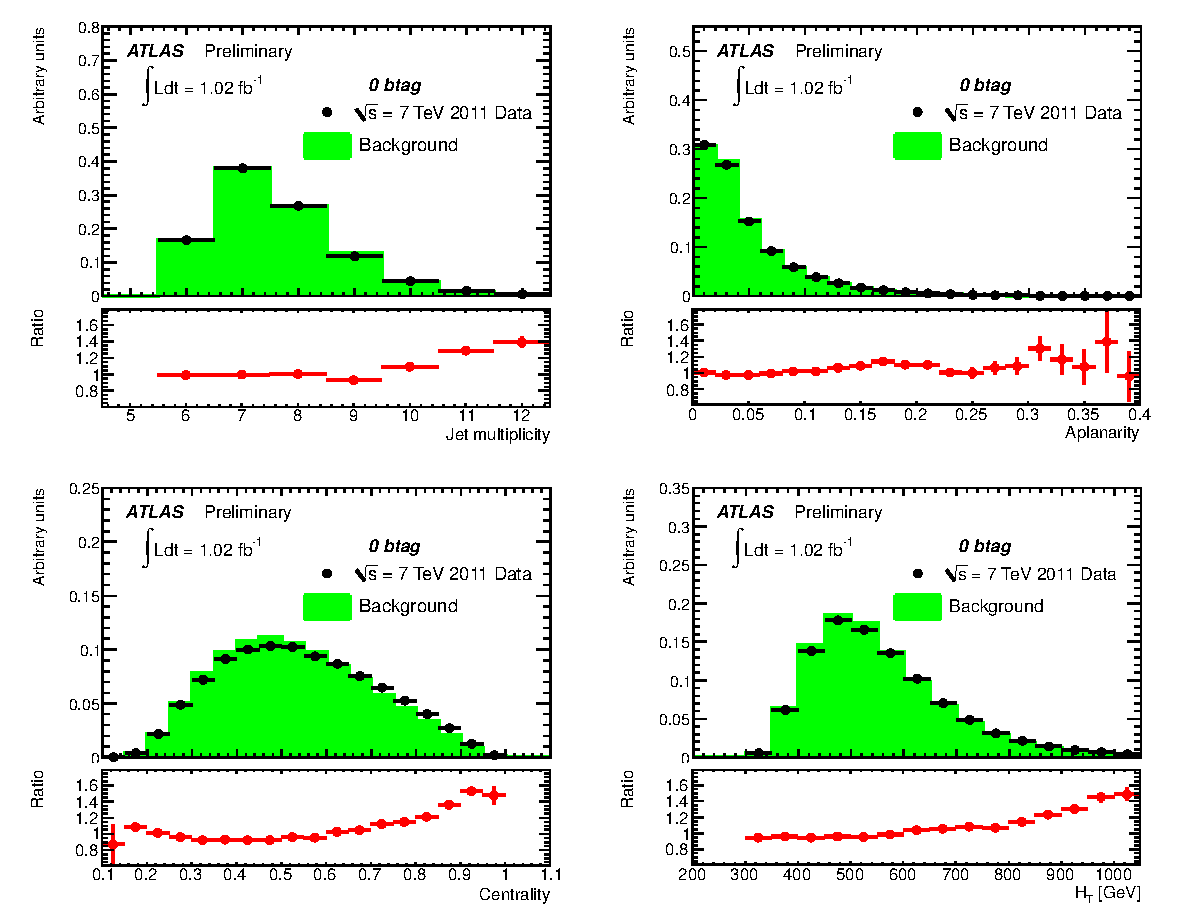
\includegraphics[width=0.95\linewidth]{figures/allhad/plot_control_5jets_0btag_ratio_24092011.eps} 
  \end{center}
  \caption{Comparison between inclusive six-jets data (dots) and the prediction modelled from five jet data for events without $b$-tagging for the number of jets, the aplanarity, the centrality and H$_T$. All histograms are normalized to have integral equal to one. Also shown the ratio between data and prediction.}
  \label{fig:control_5jets_0btag.eps}
\end{figure} 



\subsection{Systematic uncertainties and Cross-section measurement}
\label{sec:xsec}

To construct a likelihood function that separates signal from background,
a discriminating variable is constructed which resembles the $\chi^2$ of the kinematics
of an events under the signal hypothesis.
\begin{equation}
\chi^2 =  \frac{ \left(m_{j_1, j_2} - m_{W}\right)^2}{\sigma_W^2} + \frac{ \left(m_{j_1, j_2, b_1} - m_{t}\right)^2}{\sigma_t^2} + \frac{ \left(m_{j_3, j_4} - m_{W}\right)^2}{\sigma_W^2} + \frac{ \left(m_{j_3, j_4, b_2} - m_{t}\right)^2}{\sigma_t^2}, 
\end{equation}

Distributions for this variable are estimated for the $\ttbar$ signal using Monte Carlo simulation and for the QCD background using the EventMixing technique.
The scale and shapes of the templates for signal and background are susceptible to effects from a number of different sources.
These sources of systematic uncertainty, which are described below, effect the shapes and overall normalizations of the templates
representing the $\chi^2$ discriminating variable, and the effect of these uncertainties are incorporated into the likelihood
function using the modeling techniques of HistFactory.

%% Most of the systematic uncertainties are related to the signal modelling because the background is estimated by
%% a data-driven method. The only systematic uncertainty assigned to background is the background shape
%% modelling. For the signal $\ttbar$~MC sample, the systematic uncertainties are divided into shape and acceptance
%% effects. The relative shape and acceptance uncertainties are simultaneously taken into account.
%% The following systematic sources are considered together with an indication of whether they affect the shape or acceptance, or both:

The most important sources of systematic uncertainty in this analysis come from uncertainties on the Jet energy scale,
the efficiency of reconstructing jets based on the selection of this analysis, the resolution of reconstructed jets,
the efficiency of the multi-jet triggers, 
effects resulting from readout errors in the Liquid Argon calorimeter of ATLAS detector, 
and the energy scale of $b$-tagged jets.
In addition, a number of effects coming from the generation of the $\ttbar$ signal are considered, 
including differences seen across generators, effects of the level of parton shower considered, 
the parton distribution functions used,
and the rate of initial and final state radiation assumed.
Uncertainties on the measured amount of integrated luminosity are included, which effect the overall
normalization of the signal (but not the background, as it is derived from a data-driven technique).
Finally, the uncertainty on the background estimation is determined using a data-driven technique.
The uncertainty is estimated by comparing the shape of the QCD template in the signal region extracted
from either an exclusive 4-jet control region or an exclusive 5-jet control region separately.
The difference between these two extracted templates is taken as the size of the background uncertainty.
%% \item Background modelling [Event Mixing]:\\
%% The background-modelling systematic uncertainty is estimated using a four-jet event sample. 
%% The inclusive six-jet QCD background can be modelled with the two independent
%%   exclusive samples made respectively of four-jet events and five-jet events. The effect of the difference between the QCD inclusive six-jet sample built from the exclusive four-jet sample and the one produced from the exclusive five-jet one, is included as a systematic uncertainty in the $\ttbar$ production cross-section. This additional modelling uncertainty, illustrated in the right-hand panel of Figure \ref{fig:chi2.eps},  is applied to the analysis based on the five-jet trigger signature bin-by-bin to the $\chi^2$ template distribution obtained from the inclusive six-jet sample modelled from the exclusive five-jet sample. The change in the derived cross-section of 12.1\% is quoted as the associated systematic uncertainty.\\
%% An additional validation of the mixing method is performed trying it on the untagged five-jet data to predict the untagged six-jet data. The agreement on the $\chi^2$ is shown in the left-hand panel of Figure \ref{fig:chi2.eps}.\\
%% The dependency of the background modelling on the $|\Delta \pt|$ constraint between the two leading jets as well as for the fifth jets is checked. The $|\Delta\pt|$ constraint is varied from 1~GeV to 15~GeV and the maximal variation is found to be 2.3\%.
%% \begin{itemize}
%% \item Jet energy scale (JES) and associated uncertainty~\cite{ref:jessys}, [shape and acceptance]:\\
%% The jet energy scale and its uncertainty have been derived by combining information from test-beam data, LHC collision data and simulation. The residual differences between data and Monte Carlo simulation 
%% have been propagated through the analysis. Additional uncertainties due to the large pile-up effects in the 2011 data are included and range from 2\% to 7\% as a function of the jet $\pt$ and $|\eta|$.
%% The effect of JES systematics is estimated to be 24\%.
%% \item Jet reconstruction efficiency (JRE), [shape and acceptance]:\\
%% The difference in jet reconstruction efficiency between Monte Carlo simulation and data is propagated as a systematic uncertainty to Monte-Carlo. 
%% The effect of JRE uncertainty amounts to 0.1\%.

%% \item Jet energy resolution (JER)~\cite{ATLAS-CONF-2010-054}, [shape and acceptance]:\\
%% The simulated jets are smeared to match the jet energy resolution of the data. The uncertainty due to the resolution is estimated by varying the smearing factor according to the estimated uncertainties. The effect of JER is estimated to lead to an uncertainty of 13.5\%.

%% \item Trigger efficiency, [acceptance only]:\\
%% Events were selected with the five-jet trigger and by requiring the fifth-jet $\pt > 55$~GeV. The associated efficiency ranges from 
%% 90\% to 100\%, so a conservative 10\% systematic uncertainty is assigned to the trigger turn-on curve.

%% \item LAr readout problem, [acceptance only]: \\
%% A large fraction of the data (89.4\%) used in this analysis was collected in a period during which six out of 1524 front-end boards of the liquid Argon calorimeter could not be read out. As a consequence, in the data, events with an electron or a jet pointing in the direction of this inactive region were vetoed. The same procedure is applied to the simulated events. A corresponding systematic uncertainty is evaluated by varying the jet energy threshold by $\pm$4~GeV. The systematics on the cross-section amounts to 0.6\%.

%% \item $b$-tagging scale-factor (bSF) uncertainty, [shape and acceptance]:\\
%% To take into account possible differences in $b$-tagging efficiency between data and MC simulations, a set of scale factors parameterised as a function of jet $\pt$ and $\eta$ were applied to $b$-~,~$c$- and light-jets. These scale factors were varied individually within their maximal associated uncertainty and propagated through the analysis. The bSF systematic uncertainty leads to a 23\% uncertainty on the cross-section. This large uncertainty is due to the significant number of $c$-tagged jets, since the $c$-tagging uncertainty was conservatively assessed to be 20\% ( twice  the $b$-tag scale factor uncertainty). 
%% %This large uncertainty is due to the presence of $c$-tagged jets and the large uncertainty associated with the knowledge of 
%% %tagging them: twice

%% \item Generator and parton shower (PS) dependency [shape and acceptance]:\\
%% The uncertainty due to the modelling of the $\ttbar$ signal is quantified by replacing the  {\sc MC@NLO} Monte Carlo generator with {\sc POWHEG} and {\sc PYTHIA}~\cite{SJO-0601} for modelling the $\ttbar$ signal sample. The systematic uncertainty is estimated to be 5.4\%.

%% \item Initial and Final State Radiation (ISR and FSR), [shape and acceptance]:\\
%% The effects of variations in the amount of initial and final state radiation (ISR/FSR) were studied
%% using the {\sc AcerMC}~\cite{KER-0401} generator interfaced to {\sc PYTHIA} by varying the parameters controlling
%% ISR and FSR in a range consistent with experimental data. The systematic uncertainty is taken as half the maximum difference between any two samples. It amounts to 23\%.
%% %% The effects of variations in the amount of initial and final state radiation (ISR/FSR) were studied
%% %% using the AcerMC generator interfaced to PYTHIA  by varying the parameters controlling
%% %% ISR and FSR in a range consistent with experimental data. The maximum difference
%% %% between pairs of samples with reduced and increased ISR and FSR is taked as the final systematics. It amounts to 23.4\%.

%% \item Parton Distribution Function (PDF), [acceptance only]:\\
%% The uncertainty associated to the PDF is evaluated with CTEQ6.6 and its error sets. For each of the error settings, the final cross-section
%% is derived and the final uncertainty is calculated. The effect of PDF uncertainty amounts to 8.6\%.

%% \item Luminosity [acceptance]:\\
%% The uncertainty on the luminosity propagates linearly to the cross-section measurement, leading to a systematic uncertainty of $3.7\%$~\cite{ref:lum}. 

%% \item Background modelling [Event Mixing]:\\
%% The background-modelling systematic uncertainty is estimated using a four-jet event sample. 
%% The inclusive six-jet QCD background can be modelled with the two independent
%%   exclusive samples made respectively of four-jet events and five-jet events. The effect of the difference between the QCD inclusive six-jet sample built from the exclusive four-jet sample and the one produced from the exclusive five-jet one, is included as a systematic uncertainty in the $\ttbar$ production cross-section. This additional modelling uncertainty, illustrated in the right-hand panel of Figure \ref{fig:chi2.eps},  is applied to the analysis based on the five-jet trigger signature bin-by-bin to the $\chi^2$ template distribution obtained from the inclusive six-jet sample modelled from the exclusive five-jet sample. The change in the derived cross-section of 12.1\% is quoted as the associated systematic uncertainty.\\
%% An additional validation of the mixing method is performed trying it on the untagged five-jet data to predict the untagged six-jet data. The agreement on the $\chi^2$ is shown in the left-hand panel of Figure \ref{fig:chi2.eps}.\\
%% The dependency of the background modelling on the $|\Delta \pt|$ constraint between the two leading jets as well as for the fifth jets is checked. The $|\Delta\pt|$ constraint is varied from 1~GeV to 15~GeV and the maximal variation is found to be 2.3\%.

%% \item Background modelling [ABCD]:\\
%% The estimate of the \mj contamination derived with the ABCD
%% technique relies on the hypothesis that the centrality and
%% $\vartheta$ are uncorrelated. A specific uncertainty is then associated to this measurement.
%% Firstly, a correlation of $2\%$ between centrality and $\vartheta$ is
%% estimated from QCD \mj Monte Carlo samples. 
%% Such a correlation results in a relative uncertainty of 
%% $15\%$ on the cross-section obtained with the ABCD method.
%% Secondly, the centrality shape of background events was
%% reproduced with the Event Mixing technique using four-jet and five-jet events. The shape derived from the data with this method was compared between the \Br~\Dr~ and \Ar~\Cr~ regions.
%% The shapes are verified to agree to within about 1\%.
%% The value of  $\frac{{\rm N_{QCD}}^{C}}{{\rm N_{QCD}}^{A}}\times\frac{{\rm
%%  N_{QCD}}^{B}}{{\rm N_{QCD}}^{D}}$ is evaluated and found to be $1.05$.
%% This factor was introduced in Equation~\ref{eq:abcd-qcd} and gives a $30\%$
%% systematic effect on the cross-section. This value was taken as
%% the systematic uncertainty due to the correlation between the centrality and $\vartheta$.\\
%% \end{itemize}

The difference between the extracted templates using these two control regions is shown in figure ~\ref{fig:chi2.eps}
\begin{figure}[h!]
  \begin{center}
%    \includegraphics[width=0.35\linewidth]{figures/chi2.eps} 
    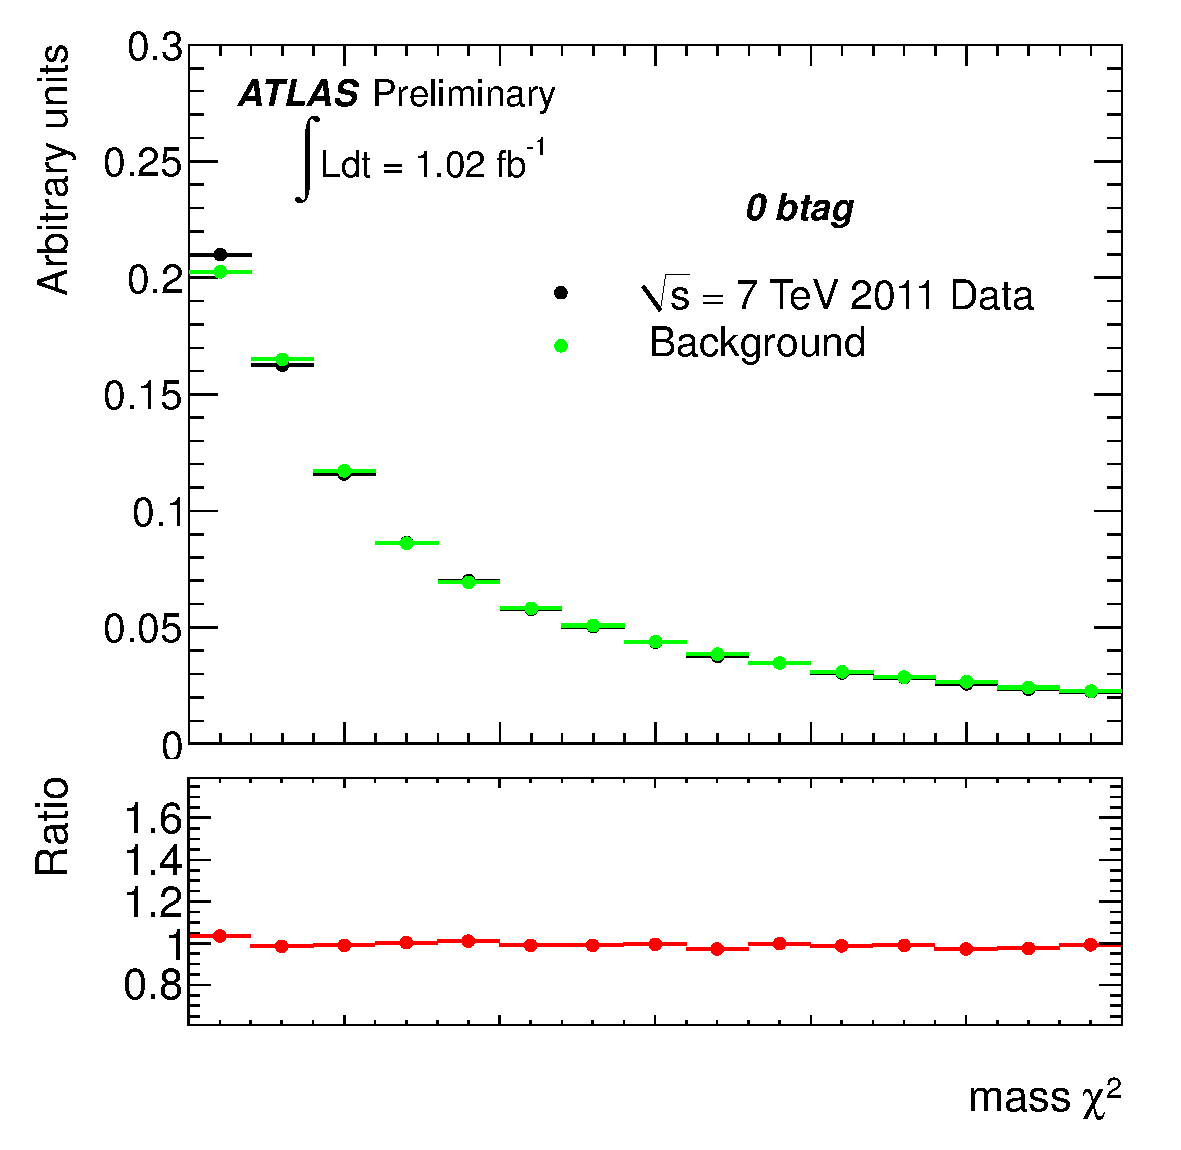
\includegraphics[width=0.45\linewidth]{figures/allhad/plot_chi2_0btag_21092011.eps} 
    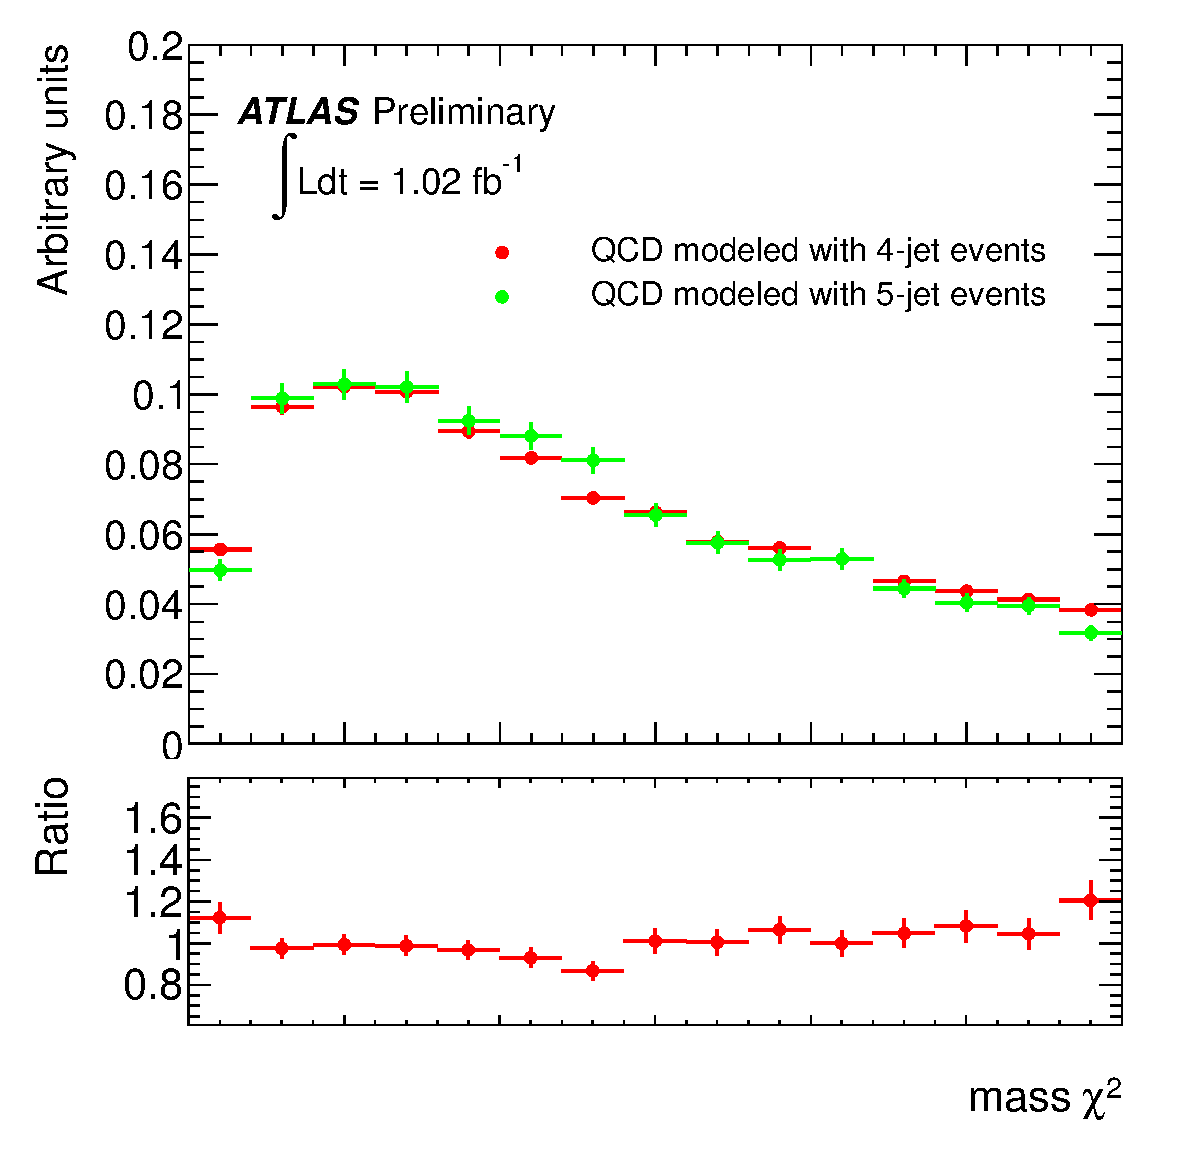
\includegraphics[width=0.45\linewidth]{figures/allhad/plot_bkgchi2_21092011.eps}\\
  \end{center}
  \caption{Left: $\chi^2$ comparison between inclusive six-jets data (dots) and the background modelled from five-jet data (green) for events without $b$-tagging. Right: comparison of the two $\chi^2$ distributions for the inclusive six-jet modelled with four-jet data (red) and the inclusive six-jet modelled with five-jet data for the four-jet trigger selected events, all events have at least two $b$-tagged jets. All histograms are normalized to have integral equal to one.}
  \label{fig:chi2.eps}
\end{figure} 
The size of the effects from systematic uncertainties are summarized in Table \ref{tab:finaluncertainties}.
\begin{table}[!h]
    \begin{center}
      \begin{tabular}{c|c}
          \hline
              \hline
              Source of uncertainty            &  Size of the effect (\%)\\
              \hline
              Jet energy scale              &          24.2    \\
              Jet reconstruction efficiency &           0.1    \\
              Jet energy resolution         &          13.5    \\
              Multi-jet trigger             &          10.0    \\
              LAr readout problem           &           0.6    \\
              $b$-tagging                   &          23.0    \\
              Generator (PS., Hadronization)&           5.4    \\
              ISR, FSR                      &          23.4    \\
              PDF                           &           8.6    \\
              Luminosity                    &           3.7    \\
              Multi-jet modelling           &          12.1    \\
              \hline
              \hline
              Total                         &          46.7    \\
              \hline
              \hline

              \end{tabular}
              \end{center}
               \caption{Summary of the different systematic uncertainties associated with the $\chi^2$
                template fit of the selected data events to the $\ttbar$ signal and \mj
                 QCD mixed sample. Uncertainties are given in \%. For the systematic uncertainties associated with the PDF, in the case of the ABCD method, the maximal variation derived from the Event Mixing based analysis is used.}
                   \label{tab:finaluncertainties}
                   \end{table}
Finally, a likelihood function is constructed that models the total distribution of the $\chi^2$ discriminant in data
as a combination of $\ttbar$ signal and QCD background.
\begin{equation}
L(f_s) = \Pi_{i} \frac{ \mu^{n_{i}} \exp(-\mu_i) }{n_{i}!}; \ \  \mu_{i} = N_{{\rm data}} \times ( f_s \times P_{i,t\bar{t}}  + (1 - f_{s}) \times P_{i,{\rm QCD}}).
\end{equation}
where $P_{t\bar{t}}$ and $P_{{\rm QCD}}$ are the fraction of $\ttbar$ and QCD events falling into the ith bin of the discriminating variable, 
$f_s$ is a parameter representing the fraction of events coming from $\ttbar$ signal, 
and $N_{{\rm data}}$ is the total number of observed events.
The $\ttbar$ cross-section is extracted by fitting this likelihood function to data while allowing the relative amount of signal to float.
The result of the likelihood fit is shown in Figure \ref{fig:fitchi2_3_Jet.eps}. 
The measured value of the top-quark pair-production cross-section is measured to be:
\begin{equation*}
 \sigma {(pp \to t\bar{t})} = 167 \pm 18 \; {\rm (stat.)} \; \pm 78 \; {\rm (syst.)} \;  \pm 6 \;  {\rm (lum.)} \; {\rm pb}
\end{equation*}
which is compatible with the Standard Model expectation of  $\sigma_{{\rm SM}} = 164^{+11} _{-16}$~pb.


%The signal content is estimated to be $f_{s}~=~$~( 24.0 $\pm$ 2.4)\% and the total $\ttbar$~cross-section $\sigma = 167 \pm 18$ (stat.) pb.

\begin{figure}[h!]
  \begin{center}
    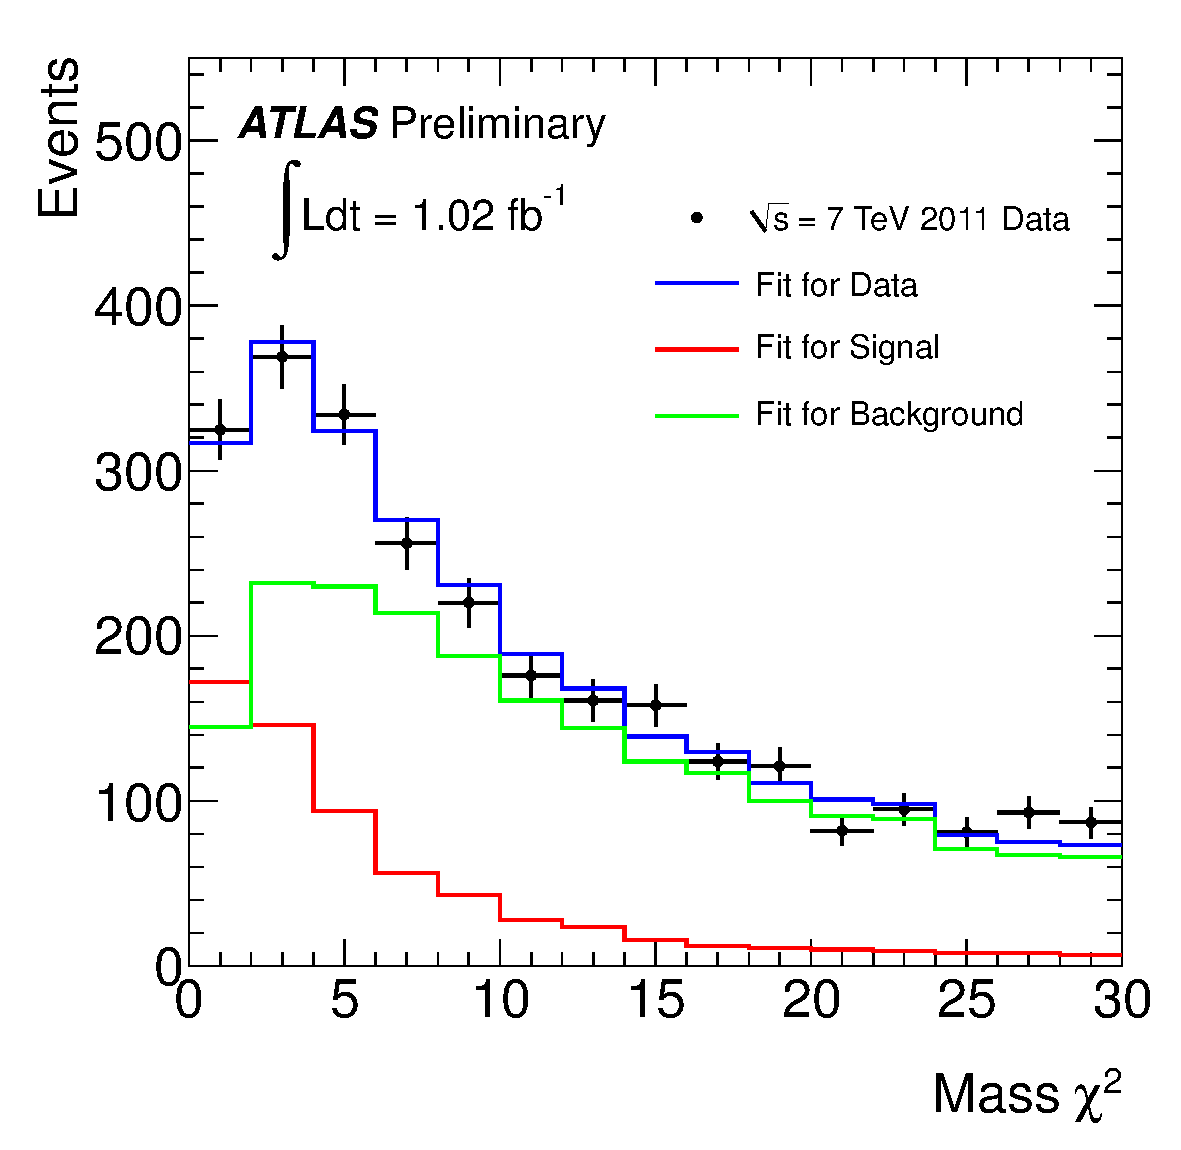
\includegraphics[width=0.75\linewidth]{figures/allhad/plot_fitchi2_21092011.eps}
  \end{center}
  \caption{Fit of the minimal mass $\chi^2$ distribution with the binned likelihood (blue line) to the selected data (dots). The $\ttbar$~signal fitted fraction is shown in red and the QCD inclusive six-jet background  in green. The errors bars associated to the data are statistical only.}
  \label{fig:fitchi2_3_Jet.eps}
\end{figure}

%% \subsection{Cross-section measurement}
%% \label{sec:xsec}

%% \noindent To test the compatibility of selected events with the $\ttbar$ hypothesis by assigning jets to the different decay products and looking at the consistency of the kinematics with the expected top quark and $W$ boson masses, a $\chi^2$-based discriminant observable was implemented. It aims to extract the $t\bar{t}$ signal from the \mj background. 

%% If there are more than two  $b$-tagged jets, the $\chi^2$ minimization chooses the two 
%% $b$-jets and the remaining $b$-tagged jets will not be used to reconstruct the $\ttbar$ system.
%% The same principle applies in the case of more than six jets where again the $\chi^2$ minimization chooses which six jets 
%% (including the two $b$-jets) will be used to form the candidate $\ttbar$ pairs.
%% The $\chi^2$ is built for each one of the six $t\bar{t}$ hypothesis. For a given event, the correct jet assignment is identified as the jet combination which minimises
%% \begin{equation}
%% \chi^2 =  \frac{ \left(m_{j_1, j_2} - m_{W}\right)^2}{\sigma_W^2} + \frac{ \left(m_{j_1, j_2, b_1} - m_{t}\right)^2}{\sigma_t^2} + \frac{ \left(m_{j_3, j_4} - m_{W}\right)^2}{\sigma_W^2} + \frac{ \left(m_{j_3, j_4, b_2} - m_{t}\right)^2}{\sigma_t^2}, 
%% \end{equation}
%% \noindent and is used to select, among the different jets, which jets to assign to each $W$ boson and top quark.
%% \noindent The $\ttbar$ signal and the background mass $\chi^2$ templates modelled respectively with MC@NLO and the Event Mixing technique described in the previous sections, are fitted to the $\chi^2$ output for the selected data events. 
%% The $\ttbar$ signal fraction and thereby the background normalization are extracted from the likelihood fit of the $\chi^2$ distribution. The likelihood is defined as:
%% \begin{equation}
%% L(f_s) = \Pi_{i} \frac{ \mu^{n_{i}} \exp(-\mu_i) }{n_{i}!}; \ \  \mu_{i} = N_{{\rm data}} \times ( f_s \times P_{i,t\bar{t}}  + (1 - f_{s}) \times P_{i,{\rm QCD}}).
%% \end{equation}
%% where $f_s$ is a parameter corresponding to the signal fraction in data and $N_{{\rm data}}$ is the number of observed data events. The symbols $P_{t\bar{t}}$ and $P_{{\rm QCD}}$ are the probabilities in the $i$-th $\chi^2$ bin extracted from the $\ttbar$ signal and QCD \mj modelled background templates. The derived number of $\ttbar$ events is then used to estimate the $\ttbar$ cross-section defined as $ \sigma_{\ttbar} = f_{s} N_{{\rm data}} / L\epsilon$, where $L$ is  the integrated luminosity and $\epsilon$, the signal selection efficiency in 
%% an inclusive $\ttbar$ sample, which includes the non all-hadronic decay modes, is estimated to be $(0.380 \pm 0.015)\%$  using the MC@NLO generator. The result of the likelihood fit is shown in Figure \ref{fig:fitchi2_3_Jet.eps}. The signal content is estimated to be $f_{s}~=~$~( 24.0 $\pm$ 2.4)\% and the total $\ttbar$~cross-section $\sigma = 167 \pm 18$ (stat.) pb.

%% Figure \ref{fig:fitchi2_4_Jet.eps} shows the top mass distribution for the selected candidates, using the jet combinations that minimize a mass $\chi^2$ in which the two $(m_{j, j, b} - m_{t})$ terms are substituted by $(m_{j_1, j_2, b_1} - m_{j_3, j_4, b_2})$, i.e. the difference between the mass of the two three-jet triplets. 
%% This $\chi^2$  does not make use of the top mass constraint, but only constrains the masses of the two triplets to be equal,
%%  allowing the mass that minimizes the term to be away from $m_{t}$.
%% For the plot shown in Figure \ref{fig:fitchi2_4_Jet.eps} the signal and background are normalized to the cross-section measured using the $m_{t}$ constraint.   


%% \begin{figure}[h!]
%%   \begin{center}
%% %    \includegraphics[width=0.8\linewidth]{figures/fitchi2_3_Jet.eps} 
%% %    \includegraphics[width=0.8\linewidth]{figures/plot_chi2Fit_07092011.eps} 
%%     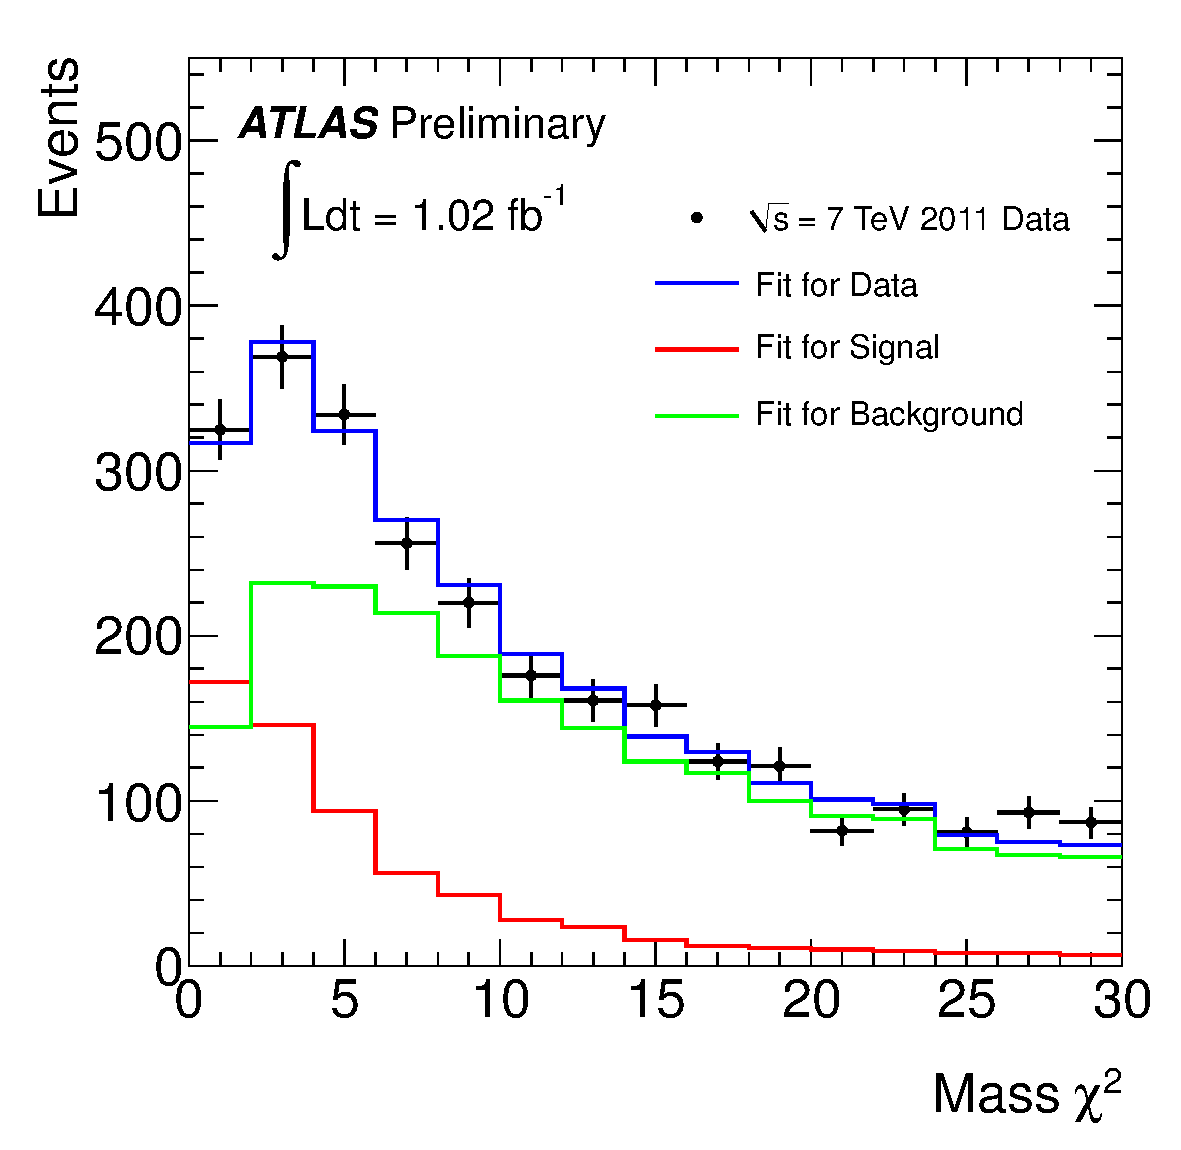
\includegraphics[width=0.75\linewidth]{figures/allhad/plot_fitchi2_21092011.eps} 
%%   \end{center}
%%   \caption{Fit of the minimal mass $\chi^2$ distribution with the binned likelihood (blue line) to the selected data (dots). The $\ttbar$~signal fitted fraction is shown in red and the QCD inclusive six-jet background  in green. The errors bars associated to the data are statistical only.}
%%   \label{fig:fitchi2_3_Jet.eps}
%% \end{figure} 

%% \begin{figure}[h!]
%%   \begin{center}
%% %    \includegraphics[width=0.8\linewidth]{figures/fitchi2_3_Jet.eps}
%% %    \includegraphics[width=0.8\linewidth]{figures/plot_chi2Fit_07092011.eps}
%%     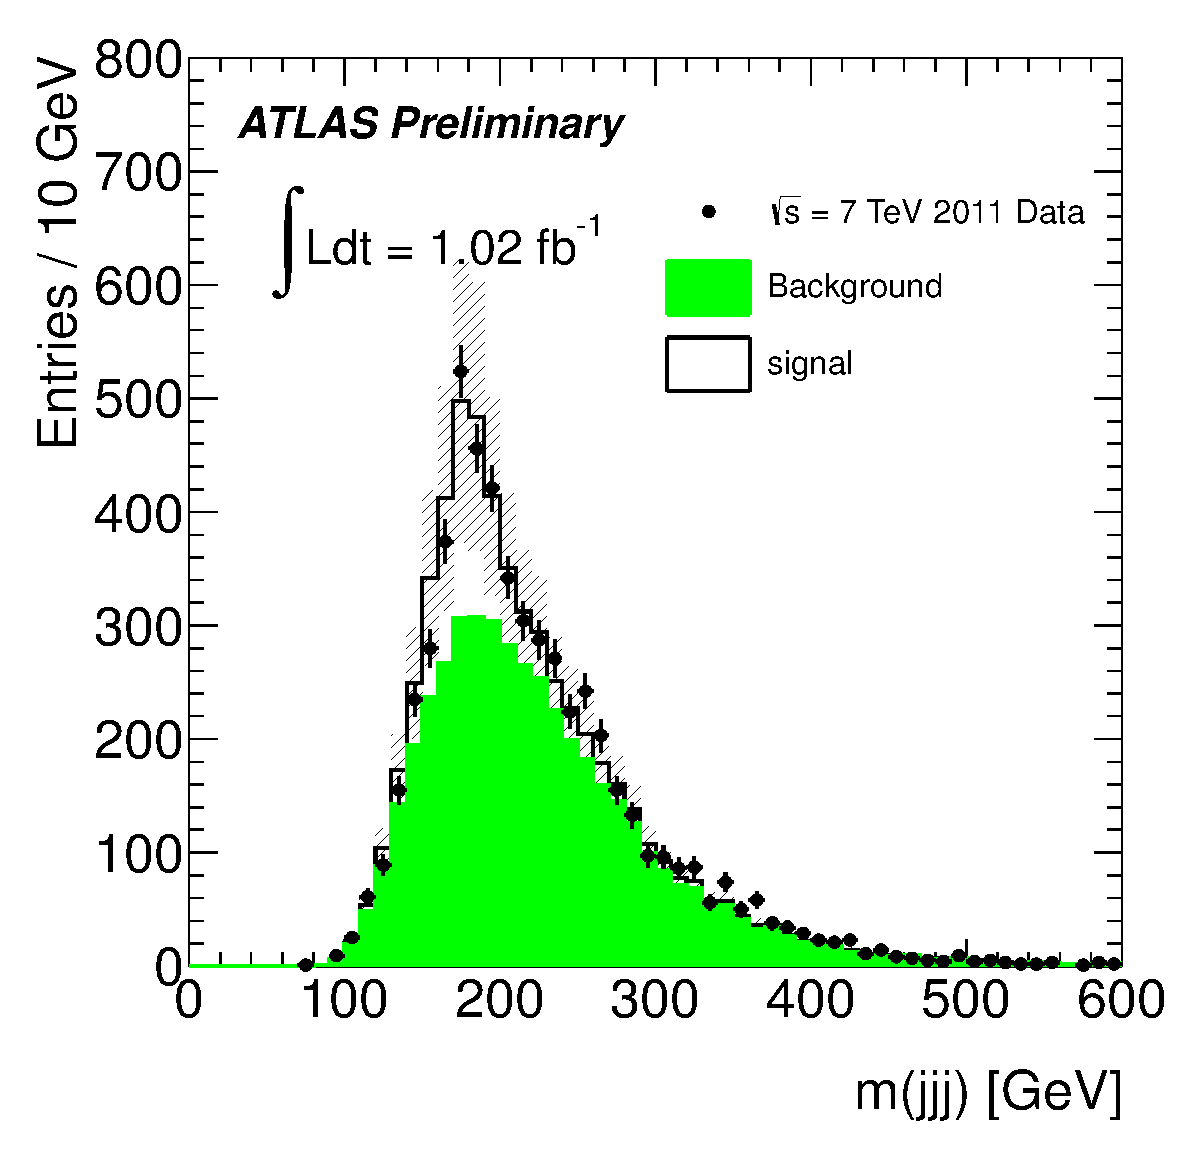
\includegraphics[width=0.75\linewidth]{figures/allhad/plot_tripletMass_172GeV.eps}
%%   \end{center}
%%   \caption{Top mass reconstructed from minimal mass $\chi^2$ distribution without top-quark mass constraint, signal and background are normalized according to the result of the fit shown in Figure \ref{fig:fitchi2_3_Jet.eps}. The errors bars represent the statistical uncertainties while the hatching represent the systematic ones. }
%%   \label{fig:fitchi2_4_Jet.eps}
%% \end{figure}



%% \subsubsection{A cross check of the Event Mixing background estimation: kinematical fit of the top mass. }
%% \label{sec:klf}

%% After performing the cross section extraction we can use a kinematic fit of the top mass as a cross check 
%% for the validity of the background modeling carried out using the Event Mixing technique. 
%% KLFitter, previously used in top analyses in the lepton plus jets channel~\cite{ATLAS-CONF-2011-033,ATLAS-CONF-2011-037}, 
%%  make use of a likelihood approach to analyze the decay of the $\ttbar$ system.  
%% Using event kinematics and the known decay chain of the top and anti-top, one is able to reconstruct the proper decay 
%% particles. The basic likelihood, which is comprised of only kinematic elements, is
%% \begin{eqnarray}
%% \rm{L_{kin}} & = &
%% \rm{BW}\left\{m(q_1 q_2) \; | \; m_W, \Gamma_W\right\} \cdot
%% \rm{BW}\left\{m(q_3 q_4) \; | \; m_W, \Gamma_W\right\} \cdot \nonumber \\
%% &&
%% \rm{BW}\left\{ m(q_1 q_2 b_1) \; | \; m_{\mathrm{top}}, \Gamma_{\mathrm{top}} \right\} \cdot
%% \rm{BW}\left\{ m(q_2 q_3 b_2) \; | \; m_{\mathrm{top}}, \Gamma_{\mathrm{top}}\right\} \cdot \nonumber \\
%% &&
%% \rm{W}\left(\tilde{E}_{\mathrm{jet}_1} \; | \; E_{b_1} \right) \cdot
%% \rm{W}\left(\tilde{E}_{\mathrm{jet}_2} \; | \; E_{b_2} \right) \cdot
%% \rm{W}\left(\tilde{E}_{\mathrm{jet}_3} \; | \; E_{q_1} \right) \cdot
%% \rm{W}\left(\tilde{E}_{\mathrm{jet}_4} \; | \; E_{q_2} \right) \cdot \nonumber \\
%% &&
%% \rm{W}\left(\tilde{E}_{\mathrm{jet}_5} \; | \; E_{q_3} \right) \cdot
%% \rm{W}\left(\tilde{E}_{\mathrm{jet}_6} \; | \; E_{q_4} \right).
%% \end{eqnarray}

%% \noindent The elements of the likelihood include Breit-Wigner components (BW) and transfer functions (W) for different p$_{T}$ 
%% and $\eta$ regions.  The likelihood describes the decay of a $\ttbar$ system.  The four Breit-Wigner fits describe 
%% the original top and anti-top quark decays into a $b$ and $W$ and the subsequent $W$ boson decays into two quarks.  
%% The transfer functions are derived from MC@NLO Monte Carlo.  To further improve the reconstruction efficiency we also include $b$-tagging information in the likelihood. 

%% For all events passing the preselection and having at least six jets within $| \eta | <$~2.5 we apply KLFitter algorithm, as well to 
%% background events modeled with the Event Mixing and Monte Carlo $\ttbar$ signal.
%% As shown in Figure~\ref{fig:klf_mass} the kinematical fit of the top mass confirms that the presence of top quark can be 
%% observed indipendently as an excess over the QCD \mj background which is consistent with the $\ttbar$ hypothesis.

%% \begin{figure}[h!]
%%   \begin{center}
%% %      \includegraphics[width=0.6\linewidth]{figures/klf_mass.eps} 
%%       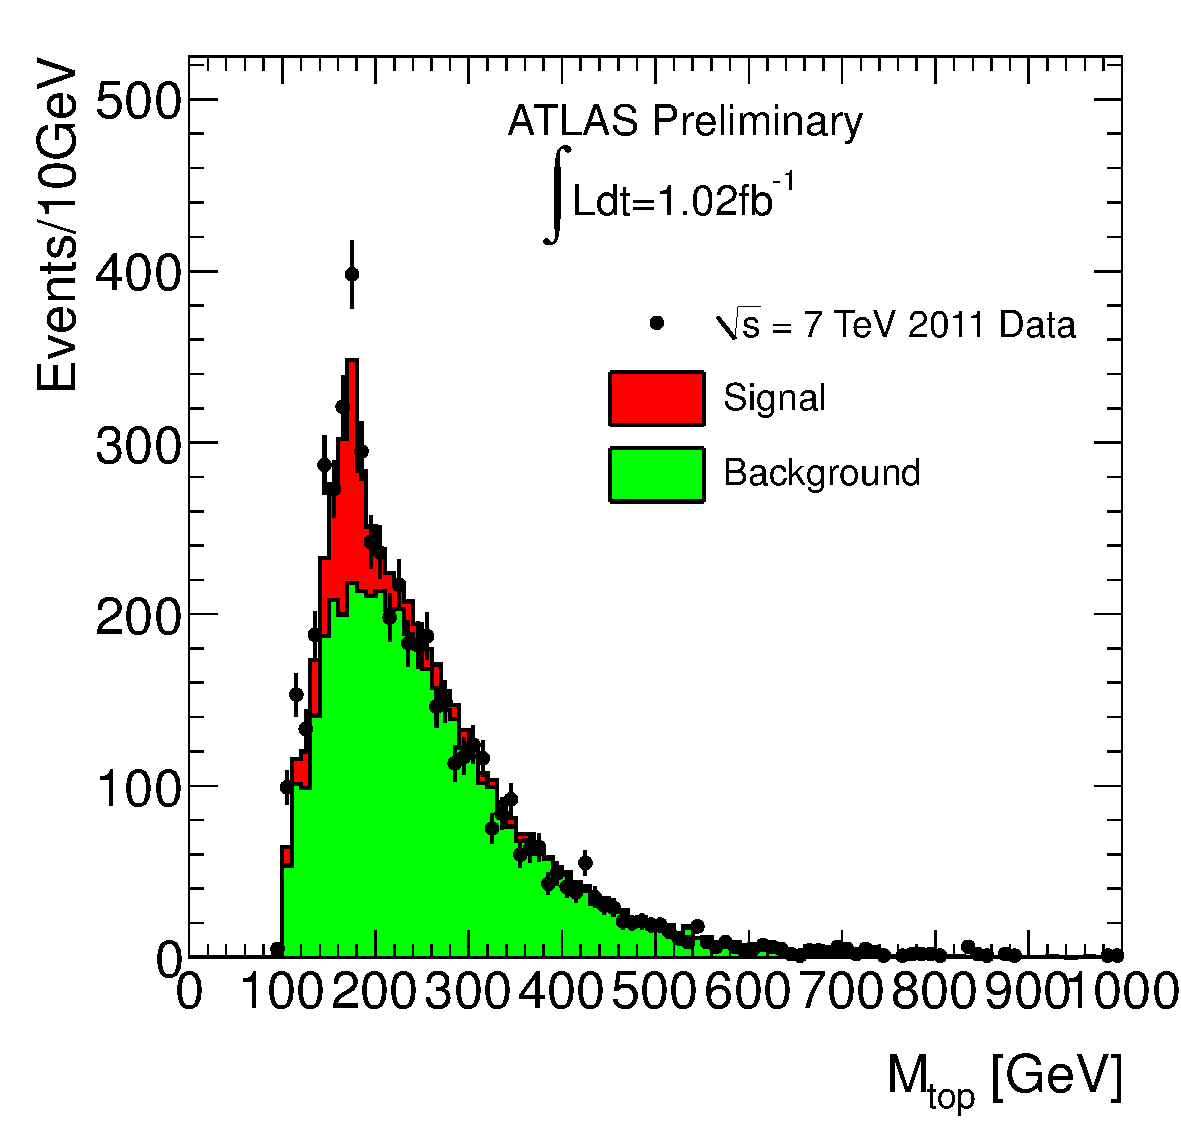
\includegraphics[width=0.6\linewidth]{figures/allhad/klf_mass_07092011.eps} 
%%       \caption{Results of the KLFitter on events passing the preselection having at least six jets within $| \eta | <$~2.5. The $t\bar{t}$ signal is normalized to the cross section measured with the likelihood fit of the $\chi^2$ distribution while the background shape is 
%%       estimated with the Event Mixing method.} 
%%   \label{fig:klf_mass}
%%   \end{center}
%% \end{figure} 



%% \subsection{ABCD analysis}

%% A second technique is used relying on a simple ABCD method, counting events in control
%% region and a signal region. The background in the signal region is extracted
%% from the yield in the control regions.

%% %These data driven approaches reduce the impact of the simulation driven systematic effects
%% %like the Monte Carlo sample size, the \mj background cross-sections and modeling.

%% \subsubsection{Background estimation}

%% %\noindent The aim of this method is to extract the observed number of \mj \ttbar
%% %events. This measurement relies on the \mj background estimation both in terms
%% %of number of events and in terms of observable shape.

%% %\noindent The ABCD method relies on the shape conservation of a selection observable when another set of uncorrelated variables is used
%% % to select the events. The following couple of variables which are assumed to be uncorrelated is used~:
%% %\begin{itemize}
%% %   \item The event centrality ;
%% %   \item The presence of at least two b-tagged jets verifying ${\Delta}R_{b\bar{b}}$.
%% %\end{itemize}

%% \noindent  Two variables are used to characterize the signal: the centrality
%%  of the event and $\vartheta$ which is defined as follows~:
%% \begin{itemize}
%%   \item $\vartheta=1$ if the event contains at least two b-tagged jets
%%   verifying $\Delta R > 1.2$
%%   \item $\vartheta=0$ if the event does not verify the first condition but
%%   contains one b-tagged jet.
%% \end{itemize}
%% Events with no b-tagged jet are rejected. These two variables have been chosen such
%%  they are uncorrelated.

%% % The overall acceptance, $\epsilon_s$ for the signal is estimated to be about
%% % $2\%$ using the Monte Carlo simulation.
%% % The acceptance of the trigger and the b-tagging cuts are corrected
%% % according to dedicated studies~[ ].
%% % A scale factor, $k$, will describe the product of
%% % the acceptance corrections and is applied to $\epsilon_s$.



%% %\begin{table}[htbp]
%% %  \small
%% %  \centering
%% %  \begin{tabular}[]{c c  c c c c c }
%% %
%% %     Cut & Signal & \btt & \wj  &  \zj & \st &   \\    \hline 
%% %     at least 2 distant b-jets & $ $ & $ $ & $ $  &  $ $ & $ $   \\
%% %     
%% %     Centrality $> 0.6$ & $ $ & $ $ & $ $  & $ $ & $ $   \\    \hline 
%% %
%% %
%% %  \end{tabular}
%% % \caption{\small Expected number of events and selection acceptance for a
%% % luminosity of $~pb^{-1}$. The signal number of events are given assuming a
%% % production cross section of $75~pb$.}
%% % \label{tab:sel_stat} 
%% %\end{table}

%% %The correlation between these two variables is evaluated on a Monte Carlo
%% %simulation of multi-jet events and found to be about $2\%$.

%% Four independent regions are defined: a
%% signal enriched region, so called \Dr region, and three control  regions, quoted \Ar,
%% \Br and \Cr dominated by
%%  \mj background events. They are defined in table~\ref{tab:abcd_regions}
%% where the expected and the observed number of events are
%% given. Figure~\ref{fig:2d_signal_data} shows the distribution of the events in
%% the plane defined by the two variables.


%% \begin{table}[htbp]
%%   \small
%%   \centering
%%   \begin{tabular}[]{c c  c c c c c c }

%%      Sample & first variable & second variable  & $\epsilon_{i}^{tt}[\%] $ & Signal~[events] & $n_i$~[events] &  $\rho$~[\%] & ${\rm N}_i$~[events] \\    \hline 
%%      D & $\vartheta = 1$ & Centrality $> 0.65$ & $0.34$ & $501.3$ & $13.0$ & $23.5\%$ & $2466$ \\
%%      B & $\vartheta = 1$ & Centrality$ < 0.65$ & $0.36$ & $498.5$ & $16.7$  & $10.1\%$ & $6112$ \\    
%%      C & $\vartheta = 0$ & Centrality $> 0.65$ & $0.49$ & $720.7$ & $42.8$ & $7.06\%$ & $11880$ \\
%%      A & $\vartheta = 0$ & Centrality $< 0.65$ & $0.57$ & $775.5$ &  $50.3$ & $2.9\%$ & $33036$ \\ \hline


%%   \end{tabular}
%%  \caption{\small Definition of the four regions, A, B, C and D. $n_i (i=a,b,c,d)$ are the contributions of W+jet,
%%  Z+jet, single top and di-boson final states. The purities and the
%%  efficiencies, $\rho$ and $\epsilon^{t\bar{t}}$, are given for all \ttbar events,
%%  including the semileptonic decays. ${\rm N}_i$ are the observed number of events in each sample.}
%%  \label{tab:abcd_regions} 
%% \end{table}


%% \begin{figure}[h!]
%%   \begin{center}
%%     \begin{tabular}{cc}
%%       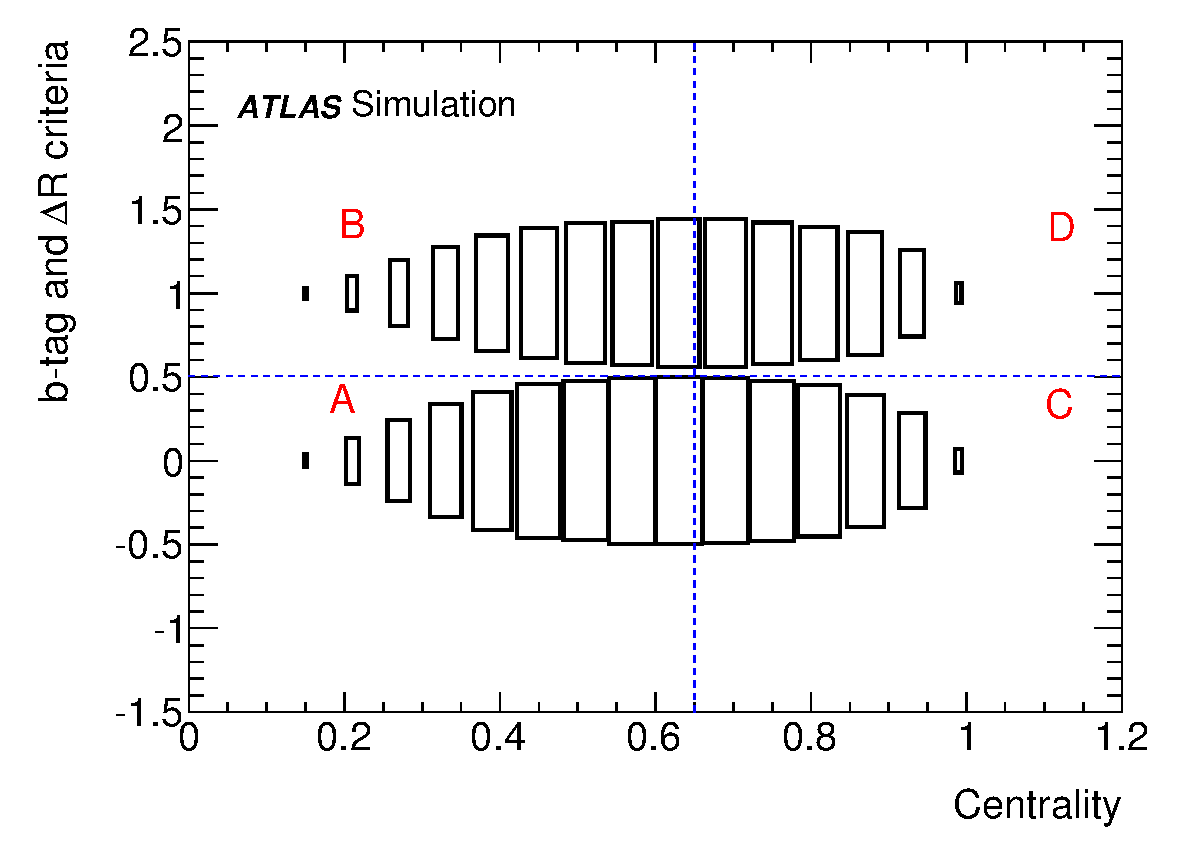
\includegraphics[width=0.4\linewidth]{figures/allhad/signal_box_abcd.eps}
%%       &  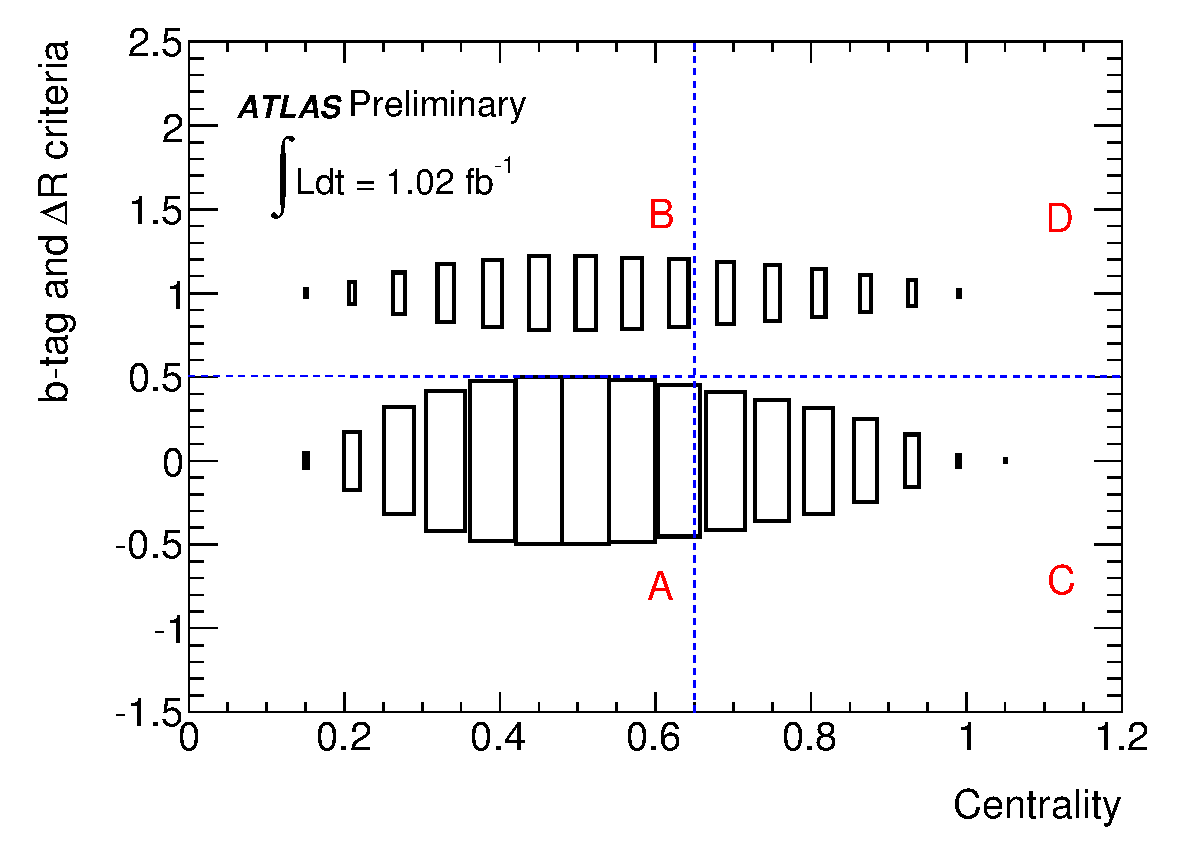
\includegraphics[width=0.4\linewidth]{figures/allhad/data_box_abcd.eps} \\
%%     \end{tabular}
%%   \end{center}
%%   \caption{Distribution of simulated signal events (left) and of data events
%%   (right) in the plane defined by the centrality and a logical variable
%%   describing the presence of at least 2 b-tagged and distant b-jets.}
%%     \label{fig:2d_signal_data}
%% \end{figure} 



%% The numbers of \mj background events in these four samples verify~:
%% $${\rm N_{QCD}^{d}} \simeq \frac{{\rm N_{QCD}}^{c}}{{\rm N_{QCD}}^{a}} {\rm
%%   N_{QCD}}^{b}$$

%% The contribution of the W+jet, Z+jet, single top and di-boson final states are
%% quoted \ba, \bb, \bc and \bd. They are estimated using the Monte Carlo simulations and
%% given in Table~\ref{tab:abcd_regions}.

%% The total number of events observed in the control samples are quoted \Na,
%% \Nb and \Nc. Assuming typical cross sections of $164~pb$ for the signal, the
%% signal fraction within in the three control
%% samples vary from $3$ to $8\%$. These signal events will then have to be taken into
%% account. 

%% The number of \mj background events in the
%% selected sample can then be written as:

%% $$ {\rm N}_{\rm QCD}(\sigma) = \left({\rm N}_{d} - n_{d} -
%%     \epsilon_{d}^{t\bar{t}}\sigma L\right) = \frac{\left({\rm
%%     N}_{b}- n_{b}-\epsilon_{b}^{t\bar{t}}\sigma L\right) \left({\rm
%%     N}_{c}- n_{c}-\epsilon_{c}^{t\bar{t}}\sigma L\right)  }{ \left({\rm
%%     N}_{a}- n_{a}-\epsilon_{a}^{t\bar{t}}\sigma L\right) } $$

%% where the acceptances $\epsilon_i^{t\bar{t}}$ ($i=a,b,c,d$) are extracted from the
%% simulation. They are defined using all the \ttbar~ decays after the multi-jet
%% selection. This second order equation involving the observed number of events and the signal
%% efficiencies only can be solved:

%% \[
%%  {\rm N}_{\rm QCD}(\sigma) = N_{d} - n_{d} - L\epsilon_{d}^{t\bar{t}} \left(
%%  \frac{-b \pm \sqrt{\Delta}}{2a} \right)
%%  \label{eq:abcd-qcd}
%% \]

%% where
%% $
%% a = L^2 \left( \epsilon_d^{t\bar{t}} \epsilon_a^{t\bar{t}} - \epsilon_b^{t\bar{t}} \epsilon_c^{t\bar{t}}  \right)
%% $, 
%% $
%% b = L \left( \epsilon_b^{t\bar{t}} (N_{c}-n_{c}) + \epsilon_c^{t\bar{t}} (N_{b}-n_{b}) - \epsilon_d^{t\bar{t}} (N_{a}-n_{a}) -
%% \epsilon_a^{t\bar{t}} (N_{d}-n_{d}) \right)
%% $, 
%% $
%% c = (N_{d}-n_{d}) (N_{a}-n_{a}) - (N_{b}-n_{b}) (N_{c}-n_{c})
%% $ and
%% $
%% \Delta = b^2 - 4ac
%% $.

%% Using the number of events shown on table~\ref{tab:abcd_regions} two solutions
%% are obtained, only one of them is positive.
%% % and equal $11212 \pm 295$
%% %events. This uncertainty is statistical only.

%% \subsubsection{Signal extraction and cross section measurement}

%% Using the formulae~\ref{eq:abcd-qcd} one can deduce the signal cross-section: 

%% \[ \sigma = -\frac{b}{2a} \pm \frac{\Delta}{2a} \]

%% The statistical uncertainty on $\sigma$ is evaluated by propagating the
%% uncertainties on $N_a$, $N_b$, $N_c$ and $N_d$ to the measurement. This
%% uncertainty includes the statistical precision on the \mj background. 
%% Using the number of events given in Table~\ref{tab:abcd_regions}, the signal
%% cross-section is estimated to be $\sigma = 161.1 \pm 37.6~pb$.
%% % ($\sigma = 244,45 \pm 67,5 pb$ using the SV1 b-tagger).

%% \subsubsection{Uncertainties due to the ABCD method}

%% The estimation of the \mj contamination derived with the ABCD
%% technique relies on the uncorrelation hypothesis between the centrality and
%% $\vartheta$. In addition to the systematic effects described with the previous
%% method a specific uncertainty is associated to this measurement.
%% In one hand, a correlation of $2\%$ between the centrality and $\vartheta$ is estimated on
%%   the Monte Carlo simulation of \mj background events using Alpgen bb+nparton samples. Such a correlation
%%   propagates to the ratio $\frac{{\rm N_{QCD}}^{c}}{{\rm N_{QCD}}^{a}} {\rm 
%%   N_{QCD}}^{b}$ by an effect of $3.5\%$. 

%% In the other hand, the centrality shape of background events was
%% reproduced with the {\it Event mixing} 
%% technique using four and five jet events. The shape derived from the data with this method was compared between \Br\Dr and \Ar\Cr regions as shown on
%% Figures~\ref{fig:abcd-syste-cent-mixing}. The agreement is verified at the level of $1\%$.
%% The value of  $\frac{{\rm N_{QCD}}^{c}}{{\rm N_{QCD}}^{a}}\times\frac{{\rm
%%  N_{QCD}}^{b}}{{\rm N_{QCD}}^{d}}$ is evaluated and found to be different from 1 by $5\%$.
%% % This value is the systematic uncertainty on the subtracted \mj background.
%% This factor of $1.05$ was introduced in the equation~\ref{eq:abcd-qcd} leading to a systematic effect of $30\%$ on the cross-section.\\

%% \begin{figure}[h!]
%%   \begin{center}
%%     \begin{tabular}{cc}
%%       \includegraphics[width=0.4\linewidth]{figures/allhad/plot_centrality_ab_cd.eps}
%%       &  \includegraphics[width=0.4\linewidth]{figures/allhad/event_fraction_bd_ac.eps} \\
%%     \end{tabular}
%%   \end{center}
%%   \caption{Comparison between the centrality in the four regions
%%     using the Event mixing technique.}
%%     \label{fig:abcd-syste-cent-mixing}
%% \end{figure} 

%% \subsubsection{ABCD method}
%% The investigated effects in the case of the ABCD method, propagate to the cross section measurements through~:
%% \begin{itemize}
%%    \item Event selection acceptance;
%%    \item Background events estimate.
%% \end{itemize}

%% The estimation of the \mj contamination derived with the ABCD
%% technique relies on the uncorrelation hypothesis between the centrality et the
%% flavor content of the event. The centrality shape of background events is
%% reproduced with the {\it Event mixing} 
%% technique an can be compared between \Br\Dr and \Ar\Cr regions as
%% shown on Figure~\ref{fig:abcd-syste-cent-mixing}. The differences are
%% compatible with the correlation of $2\%$ estimated on the Monte Carlo
%% simulation of \mj events. Such a correlation propagates to the ratio $\frac{{\rm N_{QCD}}^{c}}{{\rm N_{QCD}}^{a}} {\rm
%%   N_{QCD}}^{b}$ and then to the measured cross section. Using the data-driven centrality
%% distributions, a difference in the centrality shape between the \Br\Dr and
%% \Ar\Cr regions can be quantified using the Figure~\ref{fig:abcd-syste-cent-mixing}(right).
%%  This leads to a systematic effect of $5\%$ on the subtracted \mj background and then to a
%%  systematic effect of $35\%$ on the cross-section.

%% The largest remaining uncertainties associated to the method and derived using
%% dedicated simulations as described in the previous section. They
%% arise from the jet energy scale including pileup effects
%% ($\pm_{1.8}^{1.7}\%$),  the dead LAr regions 
%% ($\pm_{1.8}^{2.4}\%$), the jet energy resolution ($\pm 1.7\%$),
%% the jet reconstruction efficiency ($\pm 0.17\%$). The impact of
%% the the modeling of initial and final state radiation systematics was derived
%% by considering different settings of the generator parameters and yields to an
%% additional systematic uncertainty of $\pm 20\%$.

%% The uncertainty on the luminosity propagates linearly to the cross-section
%% measurement leading to a systematic uncertainty of $4.5\%$. 

%% \begin{figure}[h!]
%%   \begin{center}
%%     \begin{tabular}{cc}
%%       \includegraphics[width=0.4\linewidth]{figures/plot_centrality_ab_cd.eps}
%%       &  \includegraphics[width=0.4\linewidth]{figures/event_fraction_bd_ac.eps} \\
%%     \end{tabular}
%%   \end{center}
%%   \caption{Comparison between the centrality in the four regions
%%   using the Event mixing technique.}
%%     \label{fig:abcd-syste-cent-mixing}
%% \end{figure} 

%The different contributions to the total uncertainty are reported in table \ref{tab:finaluncertainties}.
%\begin{table}
%\begin{center}
%  \begin{tabular}{c||c|c||c|c}
%    \hline
%systematics source            &  \multicolumn{2}{c||}{\mj Event mixing} & \multicolumn{2}{c}{\mj ABCD} \\
%                              & {\tt JetComb}    &{\tt SV1}& {\tt JetComb} & {\tt SV1} \\
%Jet energy scale              &          24.2    & 22.2    &  18.9 & 16.4 \\
%Jet energy Resolution         &          13.5    & 13.5    &   7.3 & 2.5 \\
%Jet reconstruction efficiency &           0.1    &  0.1    &   0.3 & 3.5 \\
%Multijet trigger              &          10.0    & 10.0    &  10.0 & 10.0 \\   
%Dead LAr region               &           0.6    &  0.6    &   0.3  & 0.4 \\ 
%b-tagging                     &          23.0    & 21.9    &  30.0 & 31.0 \\ 
%ISR, FSR                      &          23,4    & 23.4    &  10.0 & 10.2 \\
%Generator                     &           5.4    & 4.6     &  15.0 & 7.0 \\    
%PDF                           &           8.6    & 8.9     &   8.9$^\star$& 8.9$^\star$ \\
%Luminosity                    &           3.7    & 3.7     &   3.5  & 3.5 \\   
%\hline
%\mj Modeling                  &           8.1    &10.4     & 30.0 & 30.0 \\
%\hline
%\hline
%Total                         &          45.9    &44.8     &   51.3 &  49.1 \\
%\hline
%\hline
%
%
%\end{tabular}
%\end{center}
% \caption{Summary of the different systematics associated to the chisquare
% template fit of the selected data events to the $\ttbar$ signal and multijet
% QCD mixed sample. Uncertainties are given in \% and evaluated for each one of
% the two tested b-taggers. For the systematics associated to the PDF, in the case of the ABCD method, the maximal variation derived from the Event-mixing based analysis is used.}
%  \label{tab:finaluncertainties}
%\end{table}

%% \begin{table}
%% \begin{center}
%%   \begin{tabular}{c||c||c}
%%     \hline
%% systematics source            &  Event mixing &  ABCD \\
%% Jet energy scale              &          24.2    &  13.7  \\
%% Jet energy Resolution         &          13.5    &   6.8  \\
%% Jet reconstruction efficiency &           0.1    &   0.3  \\
%% Multijet trigger              &          10.0    &  10.0  \\   
%% Dead LAr region               &           0.6    &   0.3  \\ 
%% b-tagging                     &          23.0    &  30.0  \\ 
%% ISR, FSR                      &          23,4    &  10.0  \\
%% Generator                     &           5.4    &  13.0  \\    
%% PDF                           &           8.6    &   8.6$^\star$\\
%% Luminosity                    &           3.7    &   3.7  \\   
%% \hline
%% \mj Modeling                  &           8.1    & 30.0 \\
%% \hline
%% \hline
%% Total                         &          45.9    &   49.9 \\
%% \hline
%% \hline


%% \end{tabular}
%% \end{center}
%%  \caption{Summary of the different systematics associated to the chisquare
%%  template fit of the selected data events to the $\ttbar$ signal and multijet
%%  QCD mixed sample. Uncertainties are given in \% and evaluated for each one of
%%  the two tested b-taggers. For the systematics associated to the PDF, in the case of the ABCD method, the maximal variation derived from the Event-mixing based analysis is used.}
%%   \label{tab:finaluncertaintiesWITHABCD}
%% \end{table}

%% Finally, the cross section measured using the ABCD technique is $$\sigma(pp
%% \rightarrow t\bar{t}) = 161.1 \pm 37.6(stat.) \pm 80.2(syst.) \pm 6.0(lumi.) ~pb$$.



%% % the bottom input is really stupid...
%% %\input{../INT_RC_Selection/Systematics}

%% \subsection{Systematic uncertainties}
%% \label{sec:sys}

%% Most of the systematic uncertainties are related to the signal modelling because the background is estimated by
%% a data-driven method. The only systematic uncertainty assigned to background is the background shape
%% modelling. For the signal $\ttbar$~MC sample, the systematic uncertainties are divided into shape and acceptance
%% effects. The relative shape and acceptance uncertainties are simultaneously taken into account.
%% The following systematic sources are considered together with an indication of whether they affect the shape or acceptance, or both:

%% \begin{itemize}
%% \item Jet energy scale (JES) and associated uncertainty~\cite{ref:jessys}, [shape and acceptance]:\\
%% The jet energy scale and its uncertainty have been derived by combining information from test-beam data, LHC collision data and simulation. The residual differences between data and Monte Carlo simulation 
%% have been propagated through the analysis. Additional uncertainties due to the large pile-up effects in the 2011 data are included and range from 2\% to 7\% as a function of the jet $\pt$ and $|\eta|$.
%% The effect of JES systematics is estimated to be 24\%.

%% \item Jet reconstruction efficiency (JRE), [shape and acceptance]:\\
%% The difference in jet reconstruction efficiency between Monte Carlo simulation and data is propagated as a systematic uncertainty to Monte-Carlo. 
%% The effect of JRE uncertainty amounts to 0.1\%.

%% \item Jet energy resolution (JER)~\cite{ATLAS-CONF-2010-054}, [shape and acceptance]:\\
%% The simulated jets are smeared to match the jet energy resolution of the data. The uncertainty due to the resolution is estimated by varying the smearing factor according to the estimated uncertainties. The effect of JER is estimated to lead to an uncertainty of 13.5\%.

%% \item Trigger efficiency, [acceptance only]:\\
%% Events were selected with the five-jet trigger and by requiring the fifth-jet $\pt > 55$~GeV. The associated efficiency ranges from 
%% 90\% to 100\%, so a conservative 10\% systematic uncertainty is assigned to the trigger turn-on curve.

%% \item LAr readout problem, [acceptance only]: \\
%% A large fraction of the data (89.4\%) used in this analysis was collected in a period during which six out of 1524 front-end boards of the liquid Argon calorimeter could not be read out. As a consequence, in the data, events with an electron or a jet pointing in the direction of this inactive region were vetoed. The same procedure is applied to the simulated events. A corresponding systematic uncertainty is evaluated by varying the jet energy threshold by $\pm$4~GeV. The systematics on the cross-section amounts to 0.6\%.

%% \item $b$-tagging scale-factor (bSF) uncertainty, [shape and acceptance]:\\
%% To take into account possible differences in $b$-tagging efficiency between data and MC simulations, a set of scale factors parameterised as a function of jet $\pt$ and $\eta$ were applied to $b$-~,~$c$- and light-jets. These scale factors were varied individually within their maximal associated uncertainty and propagated through the analysis. The bSF systematic uncertainty leads to a 23\% uncertainty on the cross-section. This large uncertainty is due to the significant number of $c$-tagged jets, since the $c$-tagging uncertainty was conservatively assessed to be 20\% ( twice  the $b$-tag scale factor uncertainty). 
%% %This large uncertainty is due to the presence of $c$-tagged jets and the large uncertainty associated with the knowledge of 
%% %tagging them: twice

%% \item Generator and parton shower (PS) dependency [shape and acceptance]:\\
%% The uncertainty due to the modelling of the $\ttbar$ signal is quantified by replacing the  {\sc MC@NLO} Monte Carlo generator with {\sc POWHEG} and {\sc PYTHIA}~\cite{SJO-0601} for modelling the $\ttbar$ signal sample. The systematic uncertainty is estimated to be 5.4\%.

%% \item Initial and Final State Radiation (ISR and FSR), [shape and acceptance]:\\
%% The effects of variations in the amount of initial and final state radiation (ISR/FSR) were studied
%% using the {\sc AcerMC}~\cite{KER-0401} generator interfaced to {\sc PYTHIA} by varying the parameters controlling
%% ISR and FSR in a range consistent with experimental data. The systematic uncertainty is taken as half the maximum difference between any two samples. It amounts to 23\%.
%% %% The effects of variations in the amount of initial and final state radiation (ISR/FSR) were studied
%% %% using the AcerMC generator interfaced to PYTHIA  by varying the parameters controlling
%% %% ISR and FSR in a range consistent with experimental data. The maximum difference
%% %% between pairs of samples with reduced and increased ISR and FSR is taked as the final systematics. It amounts to 23.4\%.

%% \item Parton Distribution Function (PDF), [acceptance only]:\\
%% The uncertainty associated to the PDF is evaluated with CTEQ6.6 and its error sets. For each of the error settings, the final cross-section
%% is derived and the final uncertainty is calculated. The effect of PDF uncertainty amounts to 8.6\%.

%% \item Luminosity [acceptance]:\\
%% The uncertainty on the luminosity propagates linearly to the cross-section measurement, leading to a systematic uncertainty of $3.7\%$~\cite{ref:lum}. 

%% \item Background modelling [Event Mixing]:\\
%% The background-modelling systematic uncertainty is estimated using a four-jet event sample. 
%% The inclusive six-jet QCD background can be modelled with the two independent
%%   exclusive samples made respectively of four-jet events and five-jet events. The effect of the difference between the QCD inclusive six-jet sample built from the exclusive four-jet sample and the one produced from the exclusive five-jet one, is included as a systematic uncertainty in the $\ttbar$ production cross-section. This additional modelling uncertainty, illustrated in the right-hand panel of Figure \ref{fig:chi2.eps},  is applied to the analysis based on the five-jet trigger signature bin-by-bin to the $\chi^2$ template distribution obtained from the inclusive six-jet sample modelled from the exclusive five-jet sample. The change in the derived cross-section of 12.1\% is quoted as the associated systematic uncertainty.\\
%% An additional validation of the mixing method is performed trying it on the untagged five-jet data to predict the untagged six-jet data. The agreement on the $\chi^2$ is shown in the left-hand panel of Figure \ref{fig:chi2.eps}.\\
%% The dependency of the background modelling on the $|\Delta \pt|$ constraint between the two leading jets as well as for the fifth jets is checked. The $|\Delta\pt|$ constraint is varied from 1~GeV to 15~GeV and the maximal variation is found to be 2.3\%.

%% \item Background modelling [ABCD]:\\
%% The estimate of the \mj contamination derived with the ABCD
%% technique relies on the hypothesis that the centrality and
%% $\vartheta$ are uncorrelated. A specific uncertainty is then associated to this measurement.
%% Firstly, a correlation of $2\%$ between centrality and $\vartheta$ is
%% estimated from QCD \mj Monte Carlo samples. 
%% Such a correlation results in a relative uncertainty of 
%% $15\%$ on the cross-section obtained with the ABCD method.
%% Secondly, the centrality shape of background events was
%% reproduced with the Event Mixing technique using four-jet and five-jet events. The shape derived from the data with this method was compared between the \Br~\Dr~ and \Ar~\Cr~ regions.
%% The shapes are verified to agree to within about 1\%.
%% The value of  $\frac{{\rm N_{QCD}}^{C}}{{\rm N_{QCD}}^{A}}\times\frac{{\rm
%%  N_{QCD}}^{B}}{{\rm N_{QCD}}^{D}}$ is evaluated and found to be $1.05$.
%% This factor was introduced in Equation~\ref{eq:abcd-qcd} and gives a $30\%$
%% systematic effect on the cross-section. This value was taken as
%% the systematic uncertainty due to the correlation between the centrality and $\vartheta$.\\
%% \end{itemize}
%% \begin{figure}[h!]
%%   \begin{center}
%% %    \includegraphics[width=0.35\linewidth]{figures/chi2.eps} 
%%     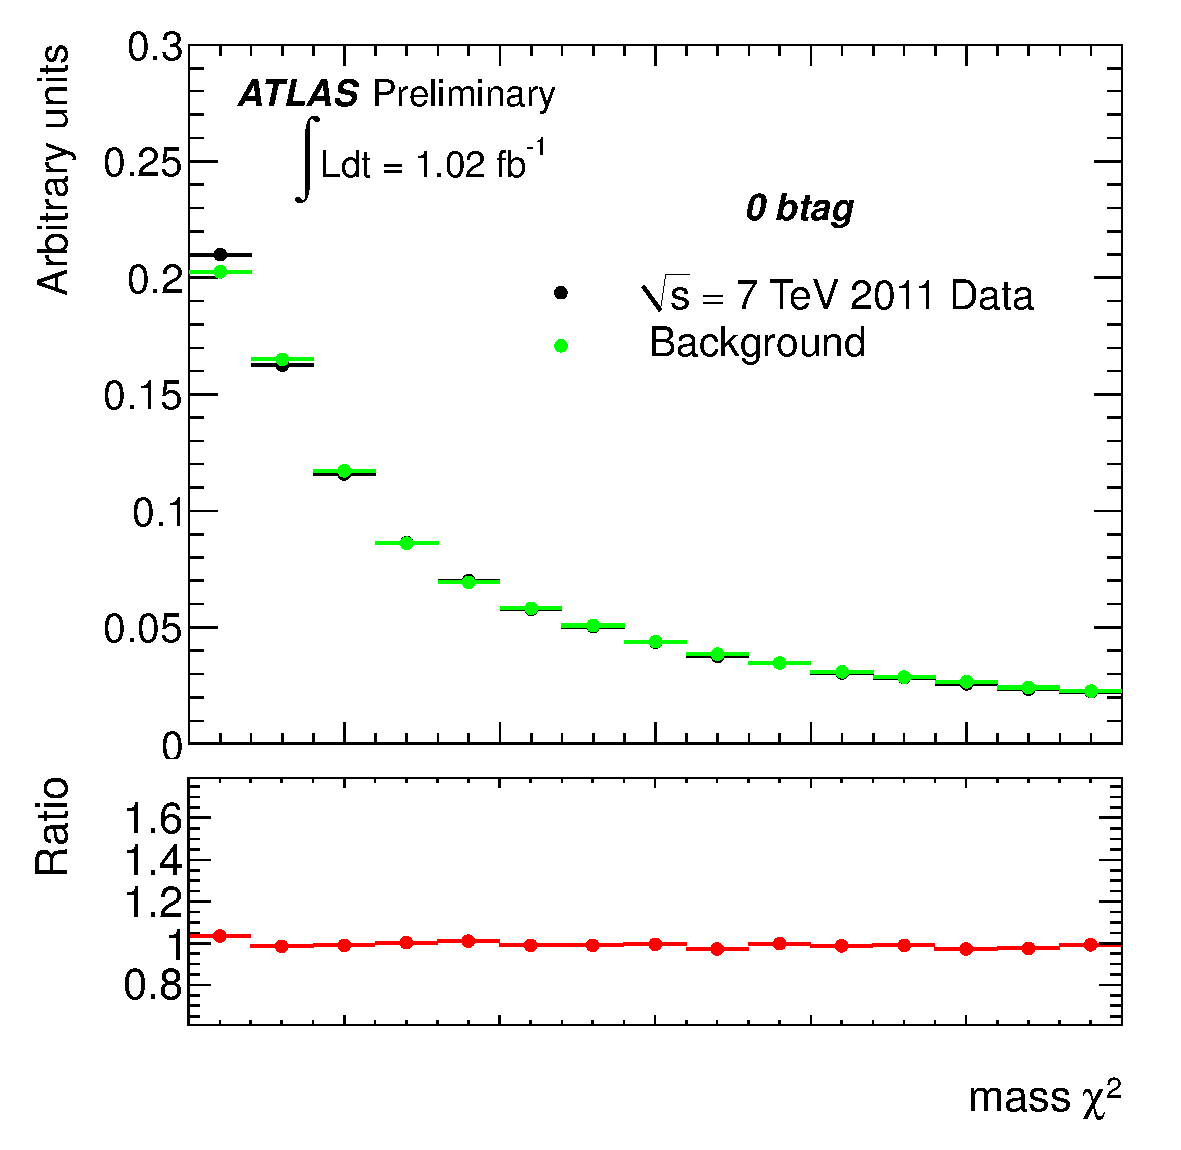
\includegraphics[width=0.45\linewidth]{figures/allhad/plot_chi2_0btag_21092011.eps} 
%%     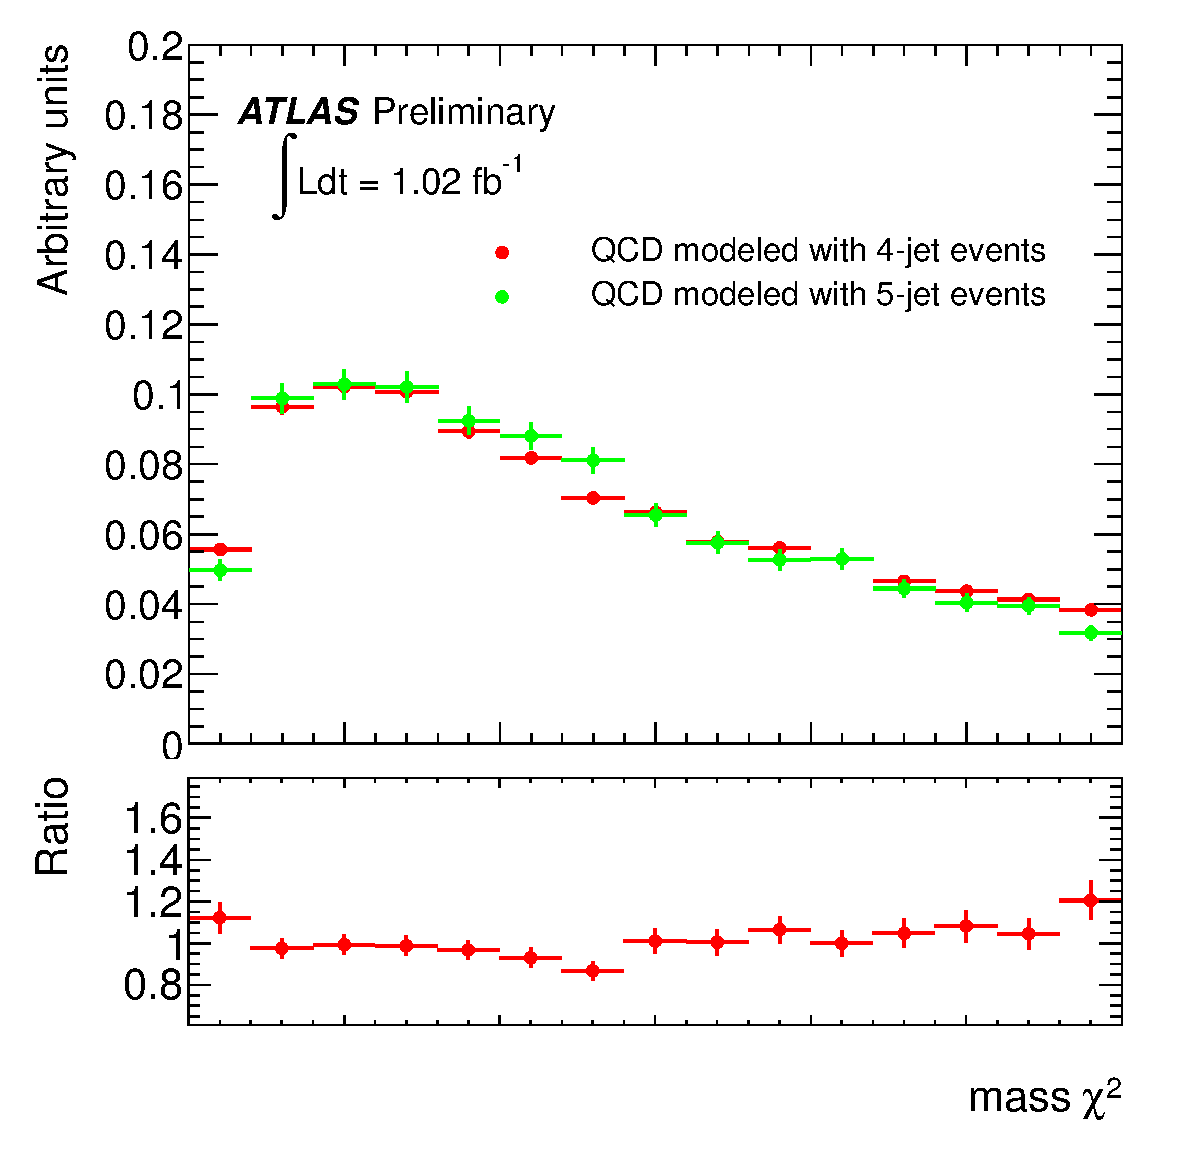
\includegraphics[width=0.45\linewidth]{figures/allhad/plot_bkgchi2_21092011.eps}\\
%%   \end{center}
%%   \caption{Left: $\chi^2$ comparison between inclusive six-jets data (dots) and the background modelled from five-jet data (green) for events without $b$-tagging. Right: comparison of the two $\chi^2$ distributions for the inclusive six-jet modelled with four-jet data (red) and the inclusive six-jet modelled with five-jet data for the four-jet trigger selected events, all events have at least two $b$-tagged jets. All histograms are normalized to have integral equal to one.}
%%   \label{fig:chi2.eps}
%% \end{figure} 

%% The systematic uncertainties are summarized in Table \ref{tab:finaluncertainties} for both the event mixing and ABCD methods. Given the lower statistical and systematic uncertainties the Event Mixing is chosen to be the main result for this note.  


%% \begin{table}[!h]
%% \begin{center}
%%   \begin{tabular}{c||c||c}
%%     \hline
%%     \hline
%% Source of uncertainty            &  Event Mixing (\%)&  ABCD (\%) \\
%% \hline
%% Jet energy scale              &          24.2    &  13.7  \\
%% Jet reconstruction efficiency &           0.1    &   0.3  \\
%% Jet energy resolution         &          13.5    &   6.8  \\
%% Multi-jet trigger             &          10.0    &  10.0  \\   
%% LAr readout problem           &           0.6    &   0.3  \\ 
%% $b$-tagging                   &          23.0    &  30.0  \\ 
%% Generator (PS., Hadronisation)&           5.4    &  13.0  \\    
%% ISR, FSR                      &          23.4    &  10.0  \\
%% PDF                           &           8.6    &   8.6\\
%% Luminosity                    &           3.7    &   3.7  \\   
%% Multi-jet modelling           &          12.1    &  30.0 \\
%% \hline
%% \hline
%% Total                         &          46.7    &   49.9 \\
%% \hline
%% \hline



%% \end{tabular}
%% \end{center}
%%  \caption{Summary of the different systematic uncertainties associated with the $\chi^2$
%%  template fit of the selected data events to the $\ttbar$ signal and \mj
%%  QCD mixed sample. Uncertainties are given in \%. For the systematic uncertainties associated with the PDF, in the case of the ABCD method, the maximal variation derived from the Event Mixing based analysis is used.}
%%   \label{tab:finaluncertainties}
%% \end{table}

% LocalWords:  QCD

%% \subsection{Summary and conclusions}
%% \label{sec:sum}

%% We have measured the production cross-section of top-antitop quark pairs in 
%% the all-hadronic decay channel at the LHC with a centre-of-mass energy of
%% $\sqrt{s}=7$~TeV and an integrated luminosity of 1.02 fb$^{-1}$ recorded with the ATLAS detector.
%% The shape of the dominant background, which consists of \mj QCD events, is modelled with a data driven technique.
%% The cross-section is extracted with a template binned likelihood fit of the event $\chi^2$ distribution:
%% \begin{equation*}
%%  \sigma {(pp \to t\bar{t})} = 167 \pm 18 \; {\rm (stat.)} \; \pm 78 \; {\rm (syst.)} \;  \pm 6 \;  {\rm (lum.)} \; {\rm pb}
%% \end{equation*}
%% which is compatible with the Standard Model expectation of  $\sigma_{{\rm SM}} = 164^{+11} _{-16}$~pb.
